\documentclass[a4paper, 11pt]{article}
% ----- Loading the Package MCMthesis -----
% -----           v 5.01-L            -----
% `tcn' is short for `Team Control Number'.
% You should fill your tcn after the equal sign following tcn.
% The option `sheet' contorls weather the summary sheet
% will appear.
% The option `abstract' controls weather the abstract 
% will appear in the title-page.
\usepackage[tcn = 1922402, sheet = true, abstract = false]{MCMthesis}
\problem{C}
\usepackage{palatino}
\setlength\parskip{.5\baselineskip}
\providecommand{\abstractname}{\relax}
\renewcommand{\abstractname}{Abstract} 

\title{MCM essay}
\author{}
\date{\today}

\begin{document}
\begin{abstract}
The first recorded Ebola outbreak occurred in Nzara, South Sudan in 1967 which infected 284 and killed 151. Since then, Ebola outbreak occurs frequently and there are nearly 20 cases of major or massive outbreaks till now, the most recent of which is the case in Liberia, Guinea and Sierra Leone in 2014. The case fatality rate ranges from 25\%(Uganda, 2007) to 90\%(Republic of Congo, 2002). Considering its high fatality rate and damage to human society, it is highly valuable to study the property of the spread of Ebola and to find out feasible strategy to fight against the virus.

In this paper, we attempted to untangle the convolution of parameters and variables concerning the spread of Ebola and to give a constructive suggestions regarding what strategy should be taken to deliver limited amount of drug and vaccine. Also, we planned to give an optimized plan to deliver vaccine and drug under a simplified case based on the real case of the recent outbreak in west Africa.

We constructed models based on the biological features of EVD, social features of human society and several reasonable assumptions. Our models consist of two parts: one is considering the the spread of disease within a single city with SIR model and serves as the base of the other; the other takes the people flow among the cities into account, the application of which gave us an optimized plan regarding how should we allocate the resources of medication such as vaccine. In fact, our model is a combination of classic SIR model and graph theory, which is a simple method to solve geography related disease spread problem.

Both of the models were applied to specific cases separately, and the results of computation which were carefully studied justified our model. Through our analysis of the model, we explored and explained the complex relationship among numerous variables and parameters. Then we find the existence of threshold values for those relationship, which indicates a limit condition for outbreak. According to the analysis and literature's instruction, we put forward our own criterion.

The effectiveness of medical treatment (including segregation, vaccination and pharmacotherapy) is verified by our model and the strategy to allocate vaccine and drug is revealed by our investigation. Specifically, the amount of vaccine or drug delivered to each city should be roughly proportional the scale of the city and the amount of vaccine or drug allocated per capita should be larger for the cities in the center of people flow network.
\end{abstract}




\maketitle
\tableofcontents
\newpage
\pagestyle{fancy}

%======================问题介绍==================
\section{Restatement of the problems}
\subsection{Background}
\par Taxi is an important way for passengers to go to the destination after getting off the plane. Passengers who want to take a taxi will go to the loading area for queuing, and then take a taxi. The airport's managers will allocate the number of passengers and taxis allowed. Domestic taxis often need to make decisions after delivering guests to the airport:

(A) go to the "car storage pool" and wait in line to take passengers and then return to the city. There is a time cost of queuing.

(B) return to the urban area without load, save the cost of queuing time, but pay the cost of no-load, and lose the potential passenger source of the airport.

For how to make decisions, drivers often judge empirically by the number of flights and passengers arriving in a certain period of time. In the real scene, there are many determinate and non determinate factors that affect the choice of drivers.

\subsection{Tasks}
\par In this paper, the mathematical model is established and the following problems are solved:

(1) find out the factors that affect the driver's judgment, including taxi revenue, number of airport passengers, etc. This paper analyzes the influence mechanism of various factors on taxi drivers, establishes the decision-making model of taxi drivers, and designs the selection strategy.

(2) collect the data of a domestic airport and related taxis, give the taxi driver's decision-making scheme in this situation, and analyze the rationality of the decision-making model built in the previous question, as well as the dependence on various factors.

(3) in the loading area, it is usually the taxi queuing to carry passengers or the passenger queuing for taxis. Now, there are two parallel lanes in the loading area. It is necessary to design the scheduling scheme of the taxi and the passenger and set the loading point so as to make the loading efficiency of the loading area the highest.

(4) there are short-distance passengers and long-distance passengers in the airport. Taxi drivers can't refuse to take them, but they can take them back and forth. In order to balance the income of all taxis, it is necessary to design a priority scheme for short-distance vehicles and verify the scheme works.
\section{Model Analysis}
In this part, we would introduce some natural characters of EVD and historical records of EVD outbreaks. This will help us understand how it spreads and determine appropriate values for the parameters in our models, such as infection rate, recovery rate, etc.

\subsection{Analysis of task 1}

\par Many factors related to Ebola influence the spread of EVD or influence the construction of our models. These factors are divided into \textbf{Social factors} and \textbf{Biological factors} and they are listed as follows.

%\subsubsection{Biological factors}
%\begin{itemize}
%  \item \textbf{Infectiousness }\\ Infectiousness directly affects the disease's infection rate, which is defined as morbidity rate for uninfected people but exposed to virus carriers. And infectiousness is mainly affected by virulence of the virus and individual's immunity. In most cases, diseases' infection rate is regarded as constant.\\ 
%      
%  \item \textbf{Lethality }\\ Lethality is how capable a disease is of causing death. It can be described by lethality rate, the ratio of the dead to the total patients. EVD has an average fatality rate of $55\%-80\%$. Moreover, Individuals who was infected and cured won't be infected again in next ten years.
%       
%  \item \textbf{Incubation}\\ Incubation means that there is a period during which the infected shows no sign or symptom of the disease and is not contagious\cite{CDC}. Therefore, there may be difficulty to segregate people with infectious diseases. EVD's incubation period is $2$ to $21$ days.
%      
%  \item \textbf{Route of Transmission} \\EVD is mainly spread through direct contact with blood and body fluids of infected ones\cite{CDC}. These routes of transmission are highly connected to public health situation and personal hygiene.
%      
%  \item \textbf{Environmental Condition}\\ Ebola virus has moderate tolerance to heat, which indicates that EVD maintains a high infectiousness in most of human settlements. However, Ebola virus will be inactivated when exposed to a temperature over $60^{\circ}$  for $60$ minutes. Environment also affects the spread of EVD in aspect of natural reservoir. Though the reservoir remains unknown, it is reasonable to infer that contact with wide animals adds to the probability of getting infected.
%      
%%  \item 
%
%\end{itemize}
%
%
%\subsubsection{Social factors}
%\begin{itemize}
%  \item \textbf{Population}\\In general, a large population means high potential of disease's spread. People in a populous area have a greater frequency of contacting the others than those in a sparsely populated area. According to the route of transmission, it is obvious that the probability of getting infected would be larger.
%   
%  \item \textbf{Traffic}\\Convinient traffic encourages population mobility, which contributes to the spread of EVD. However, It also encourages freightage, including medicine.
%  
%  \item \textbf{Medical Level}\\A society will be less affected by EVD if proper measures are taken efficiently and promptly.
%   These measures include segregating patients and strengthening the sanitary control of public places. The manufacture of drugs and vaccines aiming at EVD is also an important part.
%  
%  \item \textbf{Regional Custom}\\Funeral is considered solemn in the African culture. The dead should be cleaned, kissed and touched before buried. This kind of culture facilitates EVD infections.
%  
%  \item \textbf{Other Social Factors}\\The spread of diseases is also influenced by factors like social development, health situation, individual's living condition, etc. These factors are not considered to simplify our models.
%\end{itemize}

\subsection{Analysis of task 2}

\par In 2014, the largest outbreak of the disease occurred in West Africa, affecting multiple countries mainly including Guinea, Liberia and Sierra Leone.\cite{CDC}Up to February 4th, there have been 22,495 reported confirmed, probable, or suspected cases of EVD worldwide, with 8981 reported deaths. Among these reported cases, 99.84\% of the cases (22,460) are reported in Guinea, Liberia or Sierra Leone, thus showing a strong regional characteristic and suggesting that we should focus our study mainly within these countries.

\subsection{Analysis of task 3}

\par In 2014, the largest outbreak of the disease occurred in West Africa, affecting multiple countries mainly including Guinea, Liberia and Sierra Leone.\cite{CDC}Up to February 4th, there have been 22,495 reported confirmed, probable, or suspected cases of EVD worldwide, with 8981 reported deaths. Among these reported cases, 99.84\% of the cases (22,460) are reported in Guinea, Liberia or Sierra Leone, thus showing a strong regional characteristic and suggesting that we should focus our study mainly within these countries.

\subsection{Analysis of task 4}

\par In 2014, the largest outbreak of the disease occurred in West Africa, affecting multiple countries mainly including Guinea, Liberia and Sierra Leone.\cite{CDC}Up to February 4th, there have been 22,495 reported confirmed, probable, or suspected cases of EVD worldwide, with 8981 reported deaths. Among these reported cases, 99.84\% of the cases (22,460) are reported in Guinea, Liberia or Sierra Leone, thus showing a strong regional characteristic and suggesting that we should focus our study mainly within these countries.
\section{Model Assumptions}

%Controlling the spread of infections is by no means a new problem, and many models have previously been used to describe the distribution and spread of epidemic diseases.
%
%The models previous scientists used can mainly be divided into three categories. Brief overviews of the three by the sequence of their advent are as follows.
%\begin{enumerate}
%  \item \textbf{\emph{Standard SIR(susceptible-infected-removed) models and its deriveratives:}}The model is first put forward by \textbf{Kemraek} and \textbf{MeKendriek} in 1927\cite{SIR}and is the most classic model. Many successive models are based on it. It regards the epidemic area as a whole and divides people into different groups, such as susceptible group, infected group and removed group. It depends on differential equations to describe the relationship between volumes of different groups, thus making scientific and quantitative description. Details of the model will be explained in the successive sections.
%  \par Many other models are derived from this very basic SIR model, such as SIS model\cite{SIS} which deals with situations where a infected and later recovered individual can turn back to be a susceptible individual, and SEIR model\cite{SEIR} which deals with the situations where incubation period of the epidemic disease is not negligible. Previous scientists gained great achievements by using SIR model - they simulated the trends of epidemic diseases, calculated the rough volume of each group in different periods of epidemics and, most importantly, successfully analyse the contribution of different parameters to stability of system. 
%  \par Despite the fundamental and important standing of SIR model, its drawbacks are easy to realize. It is difficult to study geographic characters of the spread of diseases, because the model doesn't contain any geographic information. Also, each person in the system is not individually recognized and the complex relationships among individuals are hardly considered, since it regards the epidemic area as a homogeneous system - in another word, each person in the system is just like a molecule in a cup of water and the relationships of any two pairs are identical. Additionally, it is a deterministic model witch hardly resemble the factual system in which many fortuitous factors matter.
%  \item \textbf{\emph{Statistical model:}}This model is less intensely studied than the other two models. In this model, researchers mainly use possible functions whose forms are known but parameters unknown to fit the currently available data, aiming at predicting the trend of epidemics. Although the model is somewhat phenomenological and catch little intrinsic logic, it is quite useful in real practice and it allows us to have a quick view of the trend without getting convoluted into the depth of the problem. Anyhow, we will not go further into this kind of models.
%  \item \textbf{\emph{Spatial simulation model:}}This category of models are the focus recently. They mainly contains models using cellular automaton (CA), models considering networks among people(eg. small world network), models using GIS\cite{GIS}, etc. Take models using CA as an example. We define different types of points, which are put in lattices of a plane, and regard the spread of diseases between people as the interaction between nearby points. The process of evolution and spatial distribution of virus can be simulated with the aid of computer program. Clearly, due to the consideration of individuals separately, the results are more accurate than previous two categories.
%  
%  This category of models taking the relationship among people and geographic information into account has advantages over others when figuring out the geographic characters of the spread. Moreover, it can give more accurate results since its high resemblance of real situation. Accurate as the models are, they are highly complicated and some of them are difficult to apply both for the complexity of programming and great amount of computation.
%\end{enumerate}

\begin{itemize}
  \item \textbf{Population}\\In general, a large population means high potential of disease's spread. People in a populous area have a greater frequency of contacting the others than those in a sparsely populated area. According to the route of transmission, it is obvious that the probability of getting infected would be larger.
   
  \item \textbf{Traffic}\\Convinient traffic encourages population mobility, which contributes to the spread of EVD. However, It also encourages freightage, including medicine.
  
  \item \textbf{Medical Level}\\A society will be less affected by EVD if proper measures are taken efficiently and promptly.
   These measures include segregating patients and strengthening the sanitary control of public places. The manufacture of drugs and vaccines aiming at EVD is also an important part.
  
  \item \textbf{Regional Custom}\\Funeral is considered solemn in the African culture. The dead should be cleaned, kissed and touched before buried. This kind of culture facilitates EVD infections.
  
  \item \textbf{Other Social Factors}\\The spread of diseases is also influenced by factors like social development, health situation, individual's living condition, etc. These factors are not considered to simplify our models.
\end{itemize}
\section{Parameter Table}
Symbols that newly appear in this section are listed in table \ref{tab.symbol2}. Some of the symbols in table \ref{tab.symbol} are also used in this section and are not listed here.
\begin{table}[htbp]
             \centering
                \begin{tabular}{|l|l|}
                \hline
                Symbol & Defination \\
                \hline
                 $\mathcal{N}_i$ & total volume of population in city $i$\\

                $\mathcal{S}_i$ & number of susceptible people in city $i$\\

                $\mathcal{I}_i$ & number of infected but not segregated people in city $i$\\

                $\mathcal{G}_i$ & number of segregated and also infected people in city $i$\\

                $\mathcal{D}_i$ & number of death caused by EVD in city $i$\\

                $\mathcal{R}_i$ & number of recovered people (also immunized) in city $i$\\
                
                \textbf{$P_{i}$} & Total number of people in city $i$ apart from the people who are \\ & dead and segregated \\

                \textbf{$t_{i,j}$} & number of people transmit from city $i$ to city $j$ indeed \\

                \textbf{$\alpha$} & transmission coefficient \\

                \textbf{$d_{i,j}$} & distance from city $i$ to city $j$ \\
                
                $vacc_{tot}$ & the number of shares of vaccine that can be provided to all the cities every day\\
                
                $vacc_{i}$ & the number of shares of vaccine that can be provided to city $i$ every day\\
                \hline
                \end{tabular}
                \caption{The definition of the symbols.}  \label{tab.symbol2}
\end{table}

%%======================假设==================
%\subsection{Assumptions}
%\begin{itemize}
%  \item \textbf{People flow exists between any two cities }\\
%  Because no city would be quarantined totally in reality, there is connection between any two cities more or less, which means that there are flows of people between any two cities, although few people are flowing from one far-away small town to another.
%  \item \textbf{Cities are different}\\
%  To analyze the influence of delivery plan of medicines, it is better to consider that the population, location and initial status of each cities are different. To make our model realistic, we analyzed the last breakout of Ebola in west Africa in 2014 and chose some cities in the epidemic area. We consider information including geographic location, population of cities and distance between cities.
%  \item \textbf{Deterministic factors of people flow}\\
%  We assume that quantities of people leaving one city remains constant. Considering that the cities are laying on a 2-D plane, the intensity of people flow from one city to another is obviously inversely proportional to the distance between the two cities.
%  
%  We also assume that, for any individual, the probability of the one go out and link with (go to another city to visit friends, handle business affairs, etc.) any other individual are equal. Hence, it comes out that the people flow from one city to another is proportional to the product of populations of the two cities.

%  \item \textbf{Several properties of the system are time independent}\\
%To simplify our model, we assume that the quantities of drugs and vaccines delivered to each city per day are determined at the beginning and would not change with time. It means that the daily received quantity of drugs and vaccines for each city are constant. %This assumption is based on the engineering control program. Once the delivery plan has been decided, it would not change everyday because of too much sources wasting on the change.
%  
%We assume that the birth rate and natural mortality rate are generally equilibrium and fatality due to the disease is negligible compared with total population. It comes out that the total population (including fatality) is unchanging with time and the people flow among cities is also time independent.
%
%  \item \textbf{The segregated and dead would not transmit from one city to another}\\
%The S(Segregated) and D(dead due to the epidemic disease) are certainly not able to go from one city to another. Hence, when we calculated how many people from specific group are transmitted from one city to another, only the other three groups (the susceptible, the infected but not segregated, and the recovered and immunized) are taken into account.
%\end{itemize}

%\subsection{Construction of general model considering multiple cities}
%This model considering multiple cities are based on the previous single-city model. The difference between them is that in this multi-city model we consider the people flow among cities.
%
%Under assumptions previously mentioned, it is easy to conclude that the number of people transmitted from one city to another can be determined by 
%\begin{equation}
%t_{j,i} = t_{i,j}=\alpha \cdot\frac{1}{d_{i,j}}\cdot P_{i}\cdot P_{j}
%\end{equation}
%where
%\begin{equation}
%P_{i}=\mathcal{S}_{i}+\mathcal{I}_{i}+\mathcal{R}_{i}
%\end{equation}
%$\alpha$ is transmission coefficient which is a constant among all the cities, and $t_{i,j}$ is the number of people transmitted from city $i$ to city $j$.
%
%Different groups of people that are transmitted among cities are proportional to their proportion in departure city. Explicitly, for each day,
% \begin{align}\label{group}
%    \mathcal{S}_{j}&=\mathcal{S}_{j}+\sum_i \frac{\mathcal{S}_{i}}{P_{i}}\cdot t_{i,j}\\
%    \mathcal{I}{j}&=\mathcal{I}_{j}+\sum_i \frac{\mathcal{I}_{i}}{P_{i}}\cdot t_{i,j}\\
%    \mathcal{R}_{j}&=\mathcal{R}_{j}+\sum_i \frac{\mathcal{R}_{i}}{P_{i}}\cdot t_{i,j}
% \end{align}
% 
%Hence, previous derived difference equations can be written as
%\begin{subequations}
%\begin{align}
%  \dfrac{\mathcal{S}_{i+1} - \mathcal{S}_{i}}{\Delta t}&=-\frac{h}{\sigma}\mathcal{S}_i\mathcal{I}_i-\frac{vacc}{\sigma}+\sum_i \frac{\mathcal{S}_{i}}{P_{i}}\cdot t_{i,j}\\
%  \dfrac{\mathcal{I}_{i+1} - \mathcal{I}_{i}}{\Delta t}&=\frac{h}{\sigma}\mathcal{S}_i\mathcal{I}_i-\frac{(k_1+g+r_s)}{\sigma}\mathcal{I}_i+\sum_i \frac{\mathcal{I}_{i}}{P_{i}}\cdot t_{i,j}\\
%  \dfrac{\mathcal{G}_{i+1} - \mathcal{G}_{i}}{\Delta t}&=\frac{g}{\sigma}\mathcal{I}_i-\frac{k_2}{\sigma} \mathcal{G}-\frac{r_g}{\sigma} \mathcal{G}\\
%  \dfrac{\mathcal{R}_{i+1} - \mathcal{R}_{i}}{\Delta t}&=\frac{r_s}{\sigma}\mathcal{I}_i+\frac{r_d}{\sigma} \mathcal{G}_i+\sum_i \frac{\mathcal{R}_{i}}{P_{i}}\cdot t_{i,j}\\
%  \dfrac{\mathcal{D}_{i+1} - \mathcal{D}_{i}}{\Delta t}&=\frac{k1}{\sigma}\mathcal{I}_i+\frac{k_2}{\sigma} \mathcal{G}_i
%\end{align}
%\end{subequations} 
% 
%\subsection{Numerical Computation of general model considering multiple cities}
%At first, we exam the multi-city model with a simplified situation in which the quantities of drugs and vaccines delivered to each city are the same. We will show that it properly figures out the general trend of the spread of disease among cities and show us some significant character of the process.
%\subsubsection{Process of numerical computation}
%The steps of calculation are listed below:
%\begin{enumerate}
%  \item \textbf{Initial conditions}
%  \item \textbf{Calculation based on single-city model for each city }
%  \item \textbf{Simulate people flows among cities}
%  \item \textbf{Repeat Step 2 and Step 3 for the next moment}
%  \item \textbf{Until the preset $days$}
%\end{enumerate}
%In fact, from single-city model to multiple-city model, we simply added step 3.
%
%Other parameters that we are used in the computation, if not stated specifically, are the same as single-city model. For clarity, we also list them here.
%
%$\beta = 0.32$ , $k_1 = 0.023$, $r_s = 0.0103$ , $days = 150$ ,  $\Delta t = 0.1 (\text{days})$.
%
%\subsubsection{Selection of geographic data}
%Since the outbreak of EVD are usually constrained in regional areas (mentioned in background), the geographic data that we selected to simulate the last break of EVD is all from the three countries in west Africa (Guinea, Liberia and Sierra Leone). There are 145 cities in these three countries (geographic locations are plotted in figure \ref{allcity}). If all taken into account, it is not only beyond the computational ability of our computers, but also, even if results are given, is difficult for us to study the details of the results. Hence, we select 18 representative cities, among which there are big cities and also small towns; there are cities that are close to each other and there are cities far away. The data of the selected 18 cities are listed in table \ref{citylist}. For the convince of later analysis, a visualized version of data of the cities are ploted in figure \ref{cityplot}. 
%
%\begin{figure}
%\centering
%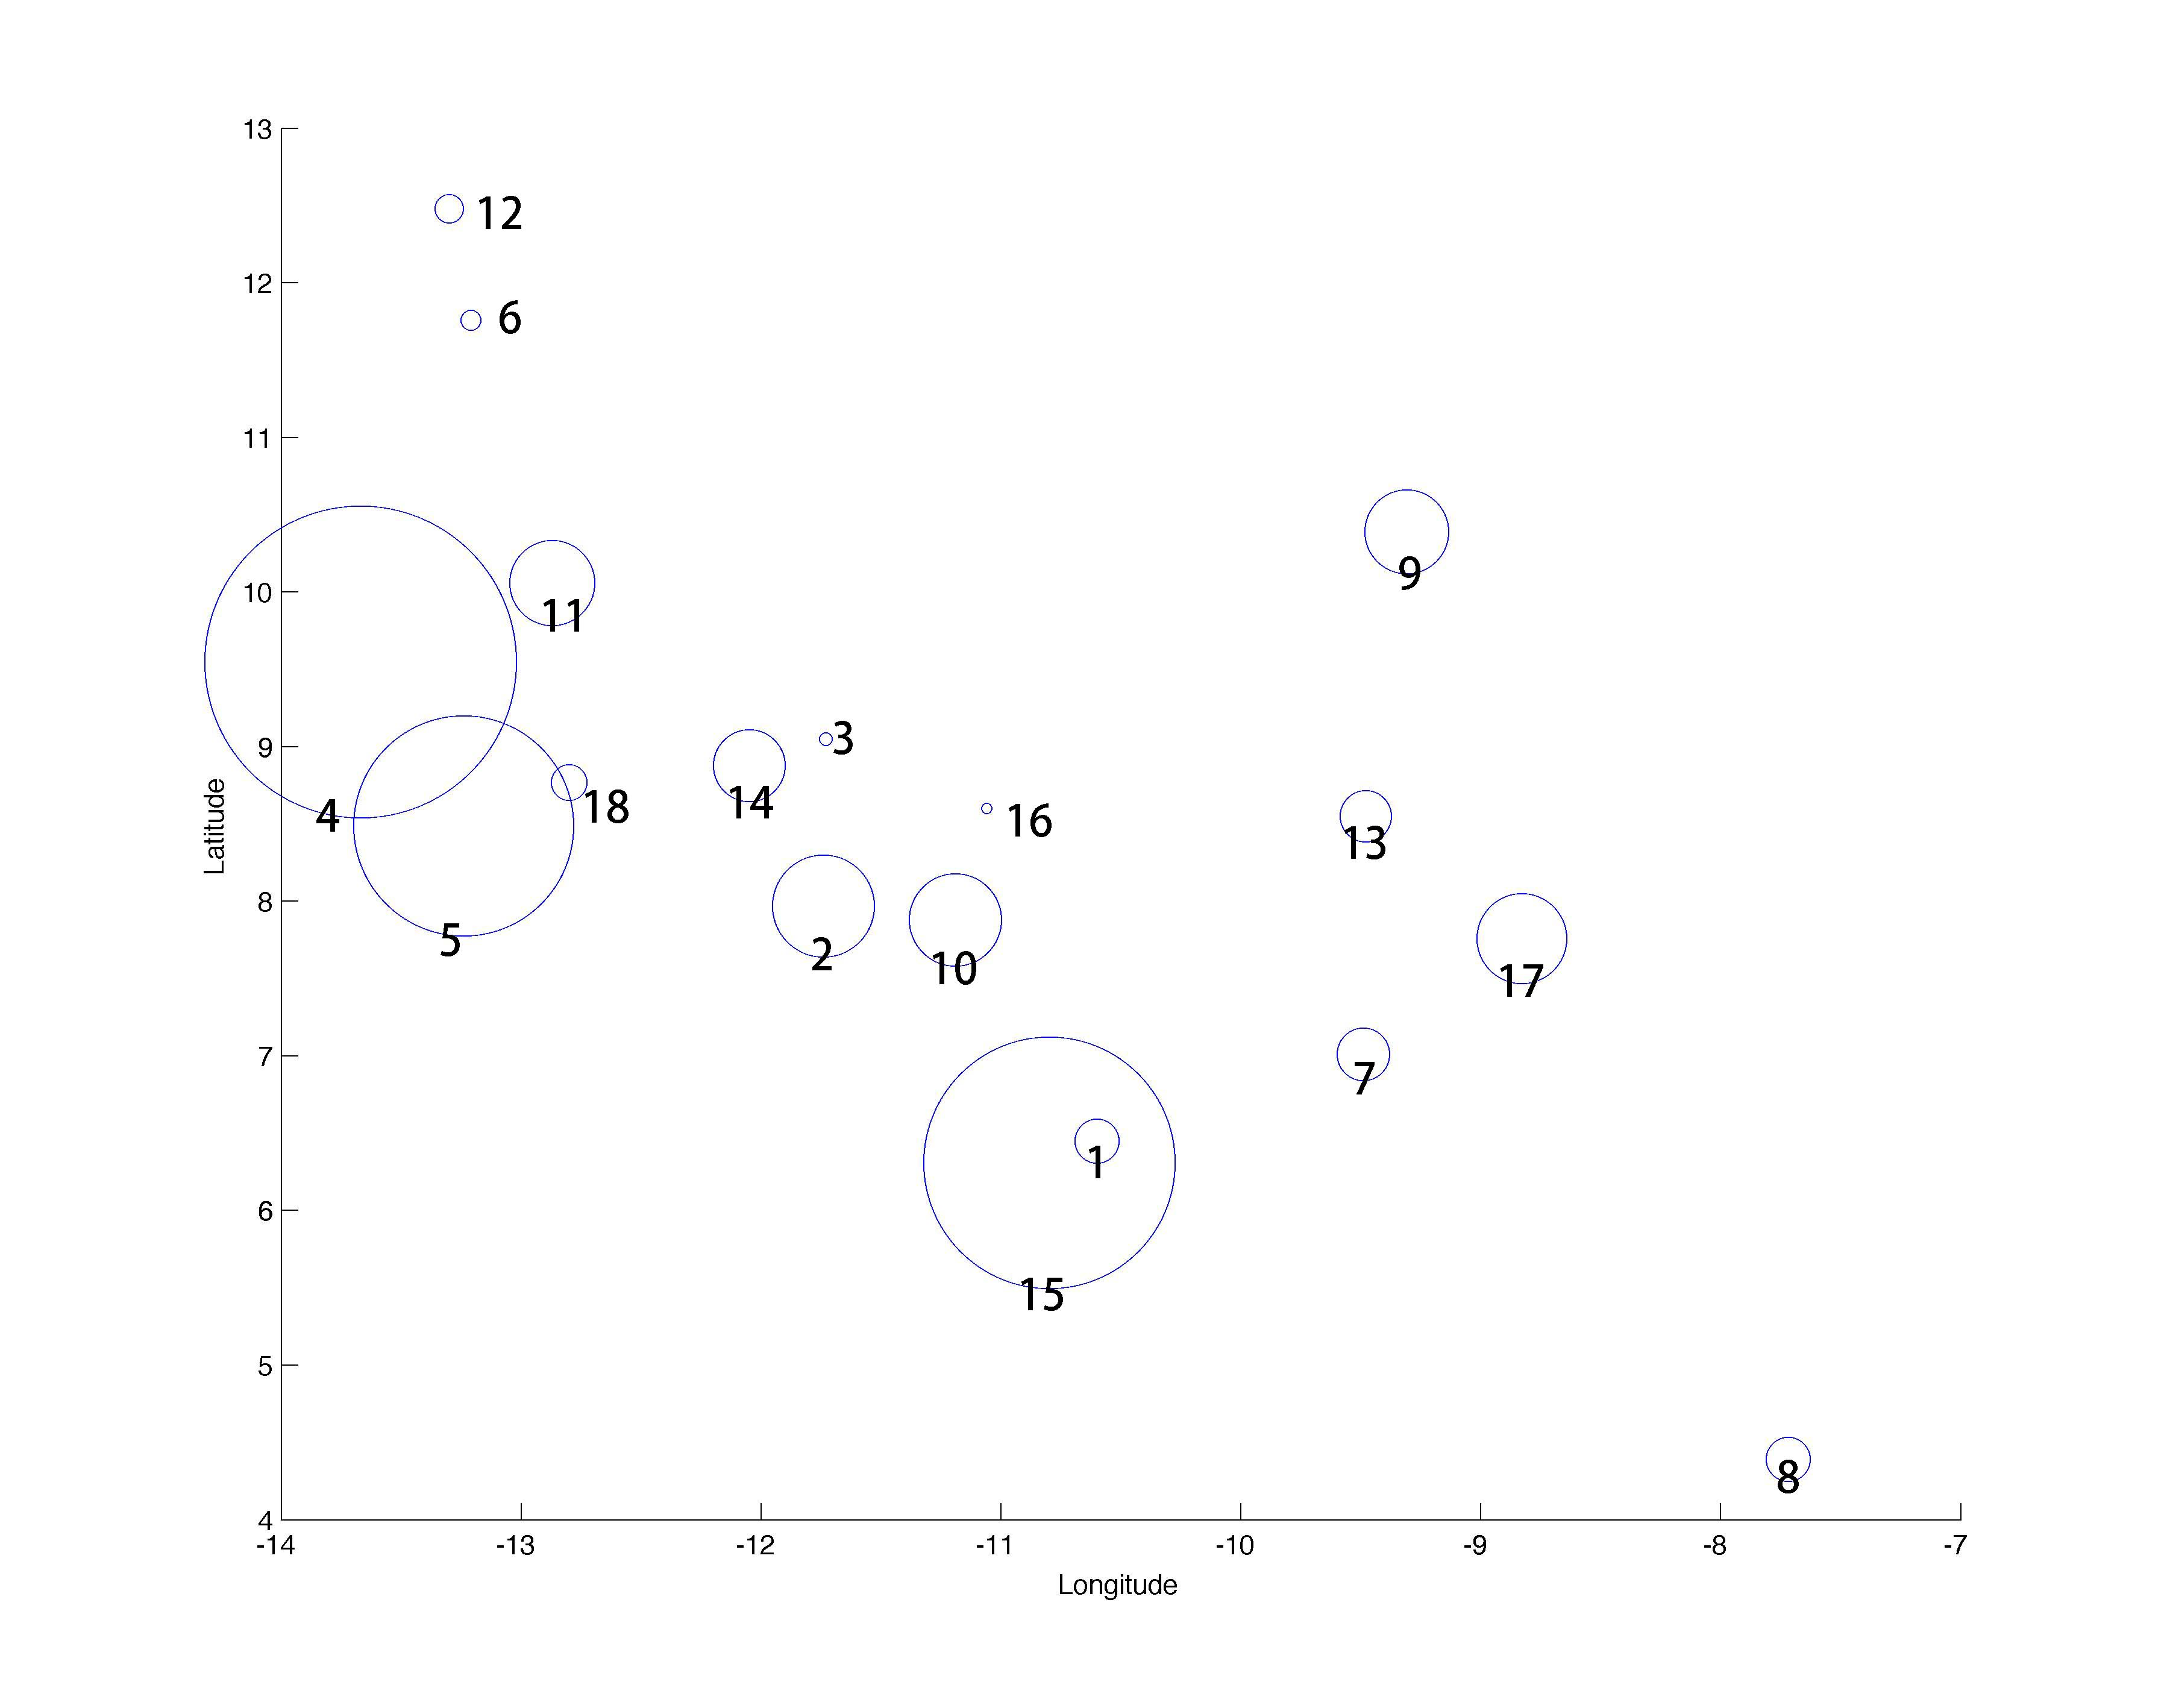
\includegraphics[width = 0.8\textwidth]{CityPopulationlabel.jpg}
%\caption{Information of 18 selected cities. Each circle stands for a city - the center of circle stands for location and the area of circle stands for population. The labels on or nearby the circles are corresponding to the labels in table \ref{citylist}}
%\label{cityplot}
%\end{figure}
%
%\begin{figure}
%\centering
%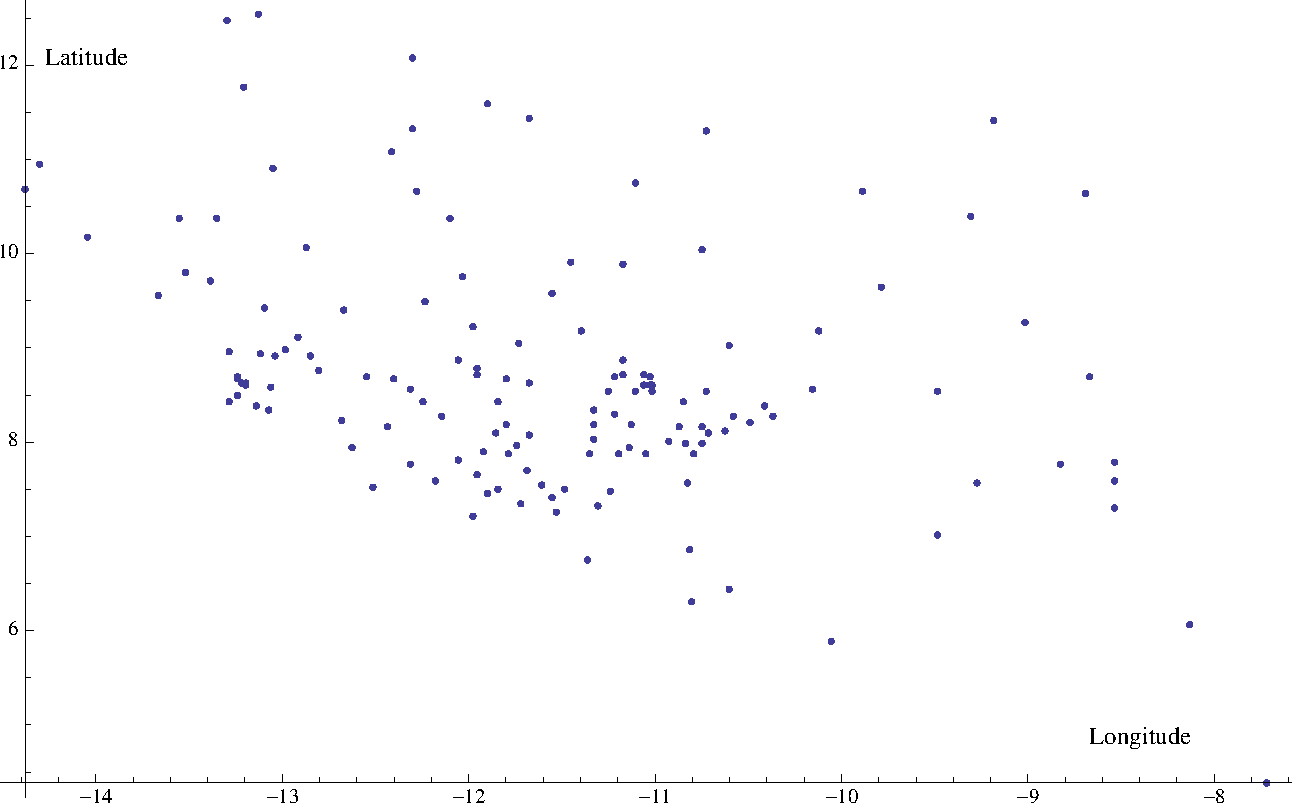
\includegraphics[width = 0.6\textwidth]{allcity.pdf}
%\caption{Locations of cities in the three countries}
%\label{allcity}
%\end{figure}
%
%\begin{table}[htb]
%\centering
%\begin{tabular}{|r|r|r|r|r|r|r|}
%    \hline
%    Label & City & Province/Region & Country & Latitude & Longitude & Population \\
%    \hline
%1 & \text{Bensonville} & \text{Montserrado} & \text{Liberia} & 6.45 & -10.6 & 33188 \\
%2& \text{Bo} & \text{Southern} & \text{SierraLeone} & 7.97 & -11.74 & 167144 \\
%3& \text{Bumbuna} & \text{Northern} & \text{SierraLeone} & 9.05 & -11.73 & 3222 \\
%4& \text{Conakry} & \text{Conakry} & \text{Guinea} & 9.55 & -13.67 & 1548470 \\
%5& \text{Freetown} & \text{Western} & \text{SierraLeone} & 8.49 & -13.24 & 772873 \\
%6&\text{Gaoual} & \text{Gaoual} & \text{Guinea} & 11.76 & -13.21 & 7461 \\
%7& \text{Gbarnga} & \text{Bong} & \text{Liberia} & 7.01 & -9.49 & 45835 \\
%8& \text{Harper} & \text{Maryland} & \text{Liberia} & 4.39 & -7.72 & 32661 \\
%9& \text{Kankan} & \text{Kankan} & \text{Guinea} & 10.39 & -9.31 & 114009 \\
%10& \text{Kenema} & \text{Eastern} & \text{SierraLeone} & 7.88 & -11.19 & 137696 \\
%11& \text{Kindia} & \text{Kindia} & \text{Guinea} & 10.06 & -12.87 & 117062 \\
%12& \text{Koundara} & \text{Koundara} & \text{Guinea} & 12.48 & -13.3 & 13990 \\
%13& \text{Macenta} & \text{Macenta} & \text{Guinea} & 8.55 & -9.48 & 43102 \\
%14& \text{Makeni} & \text{Northern} & \text{SierraLeone} & 8.88 & -12.05 & 85017 \\
%15& \text{Monrovia} & \text{Montserrado} & \text{Liberia} & 6.31 & -10.8 & 1010970 \\
%16& \text{Ndoyogbo} & \text{Eastern} & \text{SierraLeone} & 8.6 & -11.06 & 1870 \\
%17& \text{Nzerekore} & \text{Nzerekore} & \text{Guinea} & 7.76 & -8.83 & 132728 \\
%18& \text{PortLoko} & \text{Northern} & \text{SierraLeone} & 8.77 & -12.8 & 21961 \\
% \hline
%\end{tabular}
%\caption{Information of the 18 selected cities}
%\label{citylist}
%\end{table}
%
%\subsubsection{Results of numerical computation}
%Similarly, we observed both outbreak situations and well-controlled conditions when we change any one of the four independent variables($g$, $drug$, $vacc$ and $C$).
%
%Figure \ref{multibreak} shows clearly how the outbreak of disease spread from one city to another. We have observed that: 1) the order of severity (measured by fatality) is larger in the city which is the onset of disease (in our special case it is city 1) ; 2) epidemic outbreak occurs earlier in the city which is the onset of disease, in another word, the general trend of others has somewhat 'lag effect'; 3) the general trend of the city close to the onset of disease resembles more to the onset of disease in terms of severity and time sequence (in our special case it is city 15).
%
%\begin{figure}
%\centering
%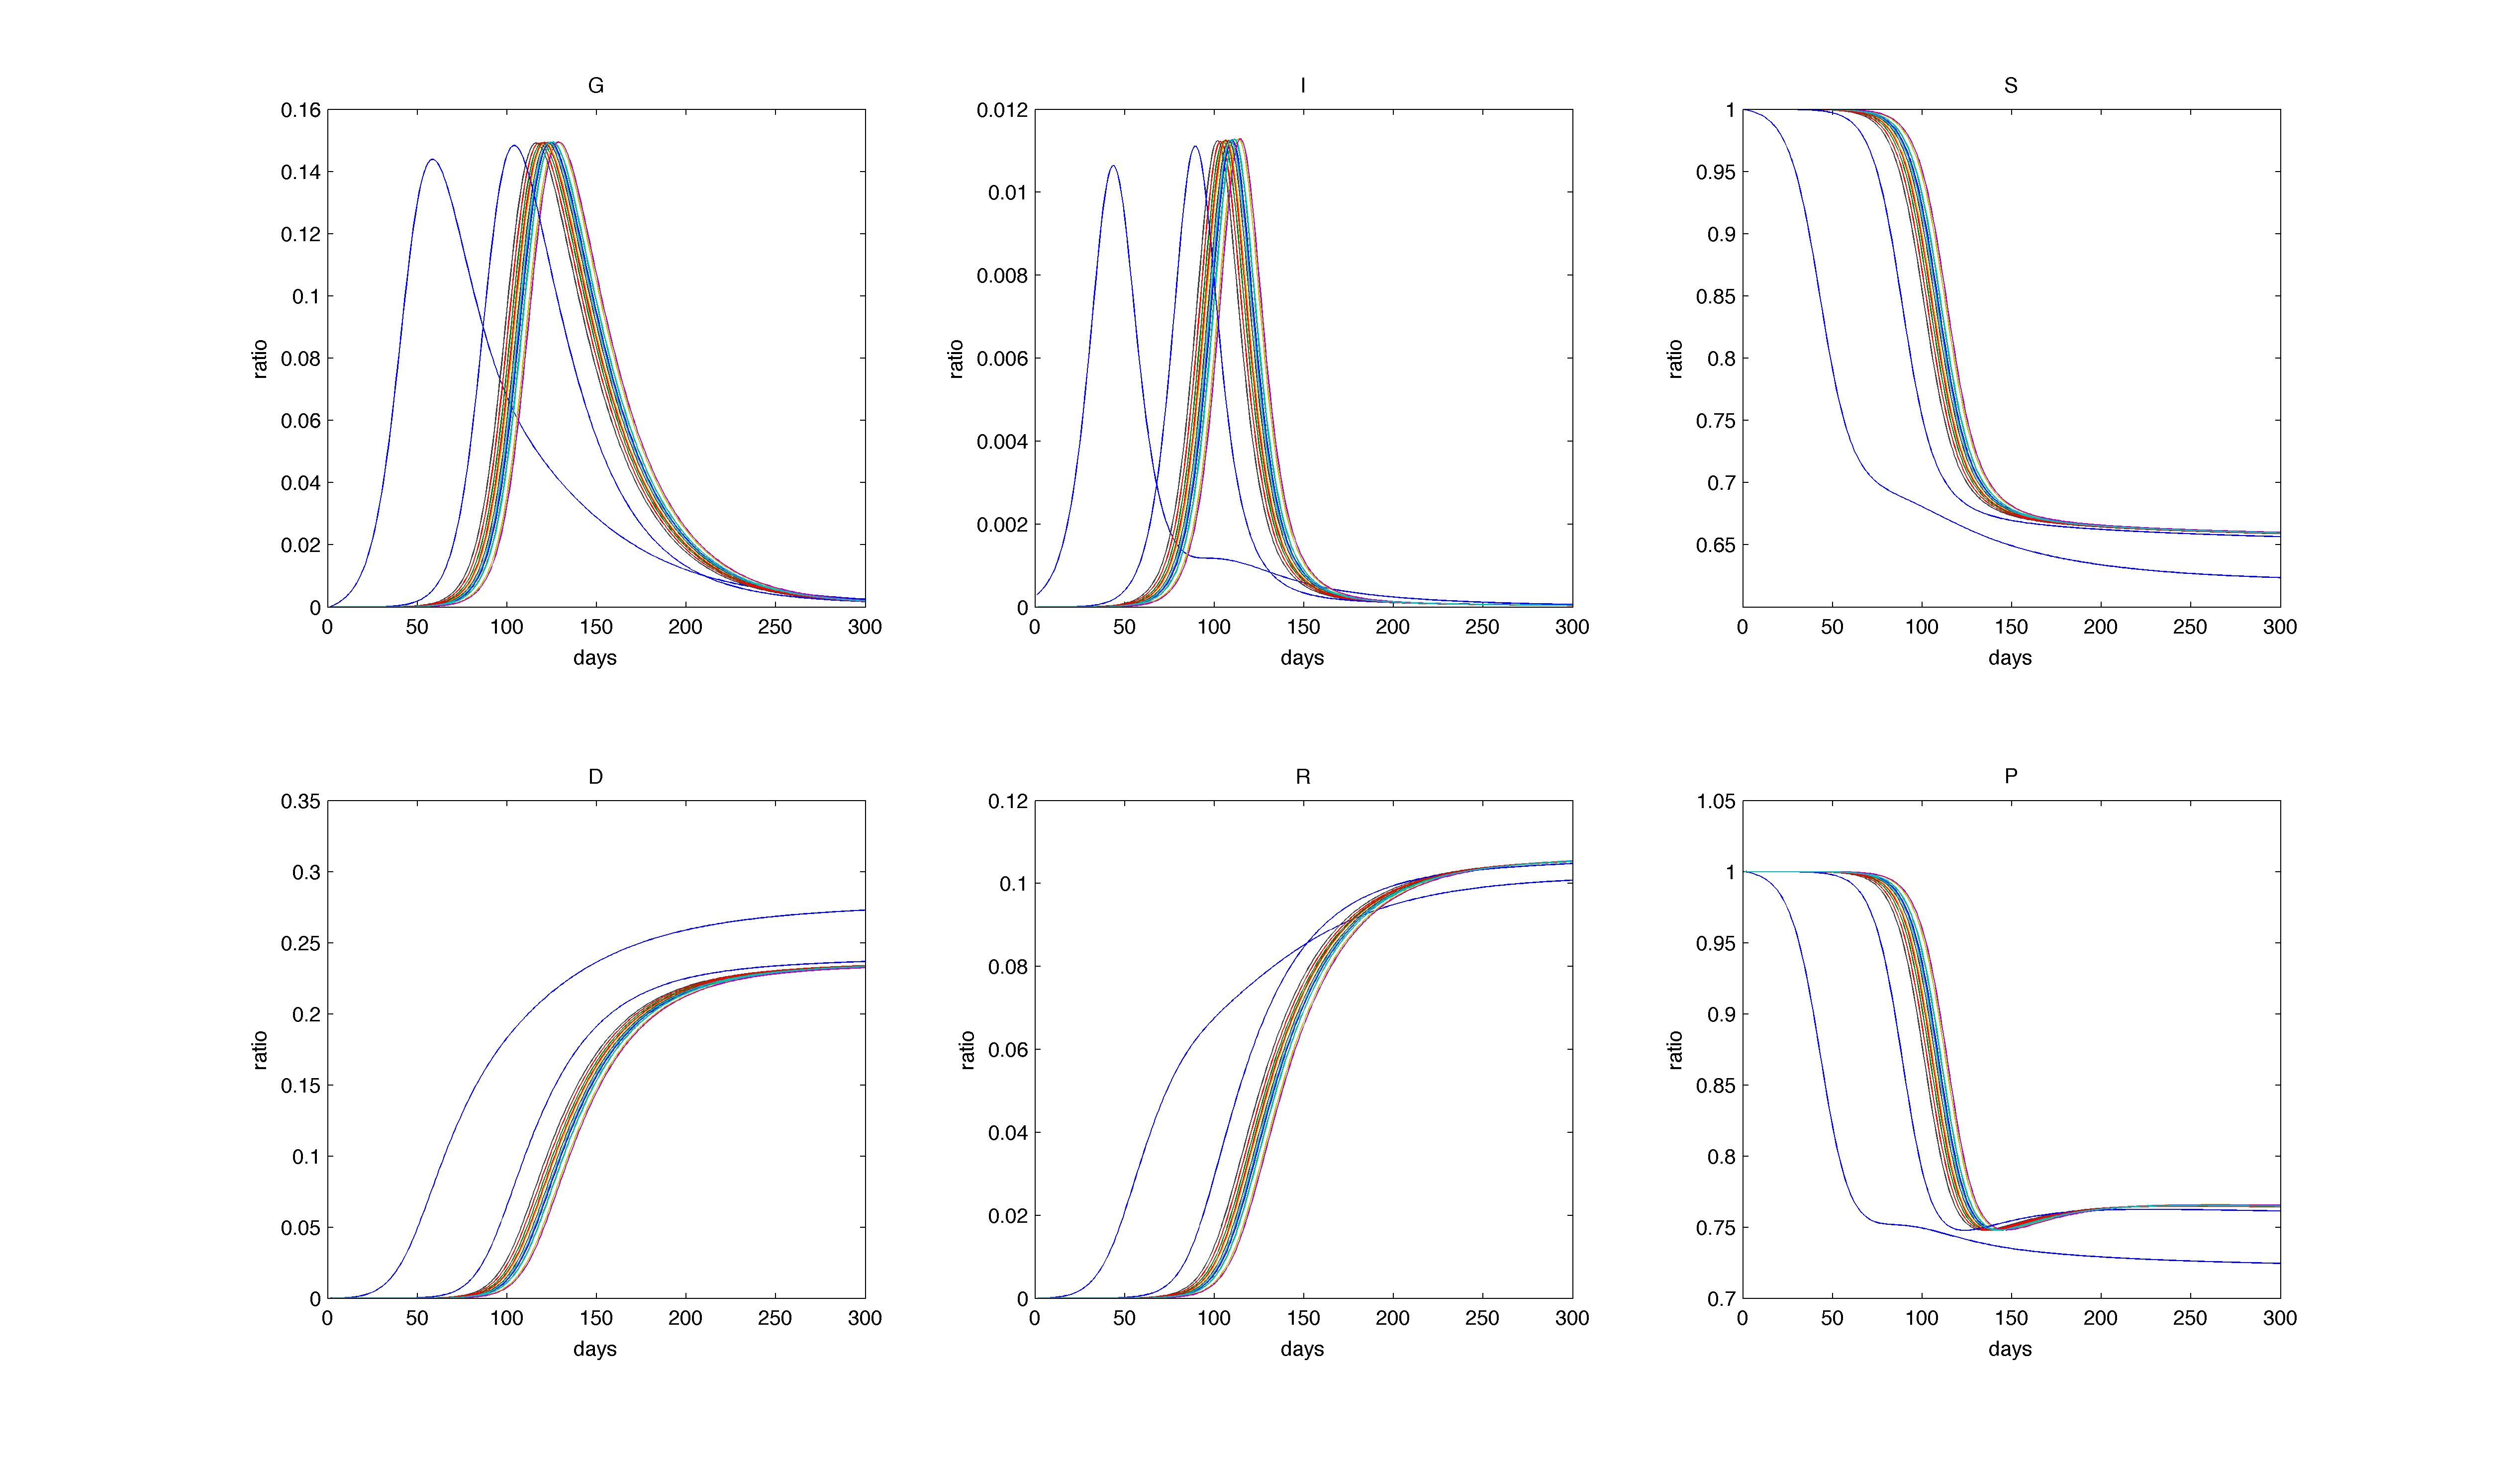
\includegraphics[width = 0.8\textwidth]{multibreak.jpg}
%\caption{epidemic disease breakout in different cities. $days = 300$, $\alpha = 10^{-4}$ , $drug = 0, vacc = 0, C = 3, g = 0.8$ and the y axis is the number of people in the group divided by the total number of people in corresponding city. Initially, 10 people are infected in city 1, and all the other people in all the cities are susceptible. The dark blue line far away from others represents city 1. The next dark blue line which is easy to distinguish from others represents city 15 which is geographically close to city 1.}
%\label{multibreak}
%\end{figure}
%
%Figure \ref{multicontrol_1000vacc} shows that when giving vaccines to the cities, the severity greatly decreases, which indicates the great influence medication has on the spread of disease. Additionally, we have observed a new phenomenon that big cities are more easy to get influenced by epidemic diseases if all the cities are given identical amount of drug or vaccine. In our special case, the trend of city 4 is showing the phenomenon. Similar features are observed when varying the value of $drug$, $C$, or $g$.
%
%\begin{figure}
%\centering
%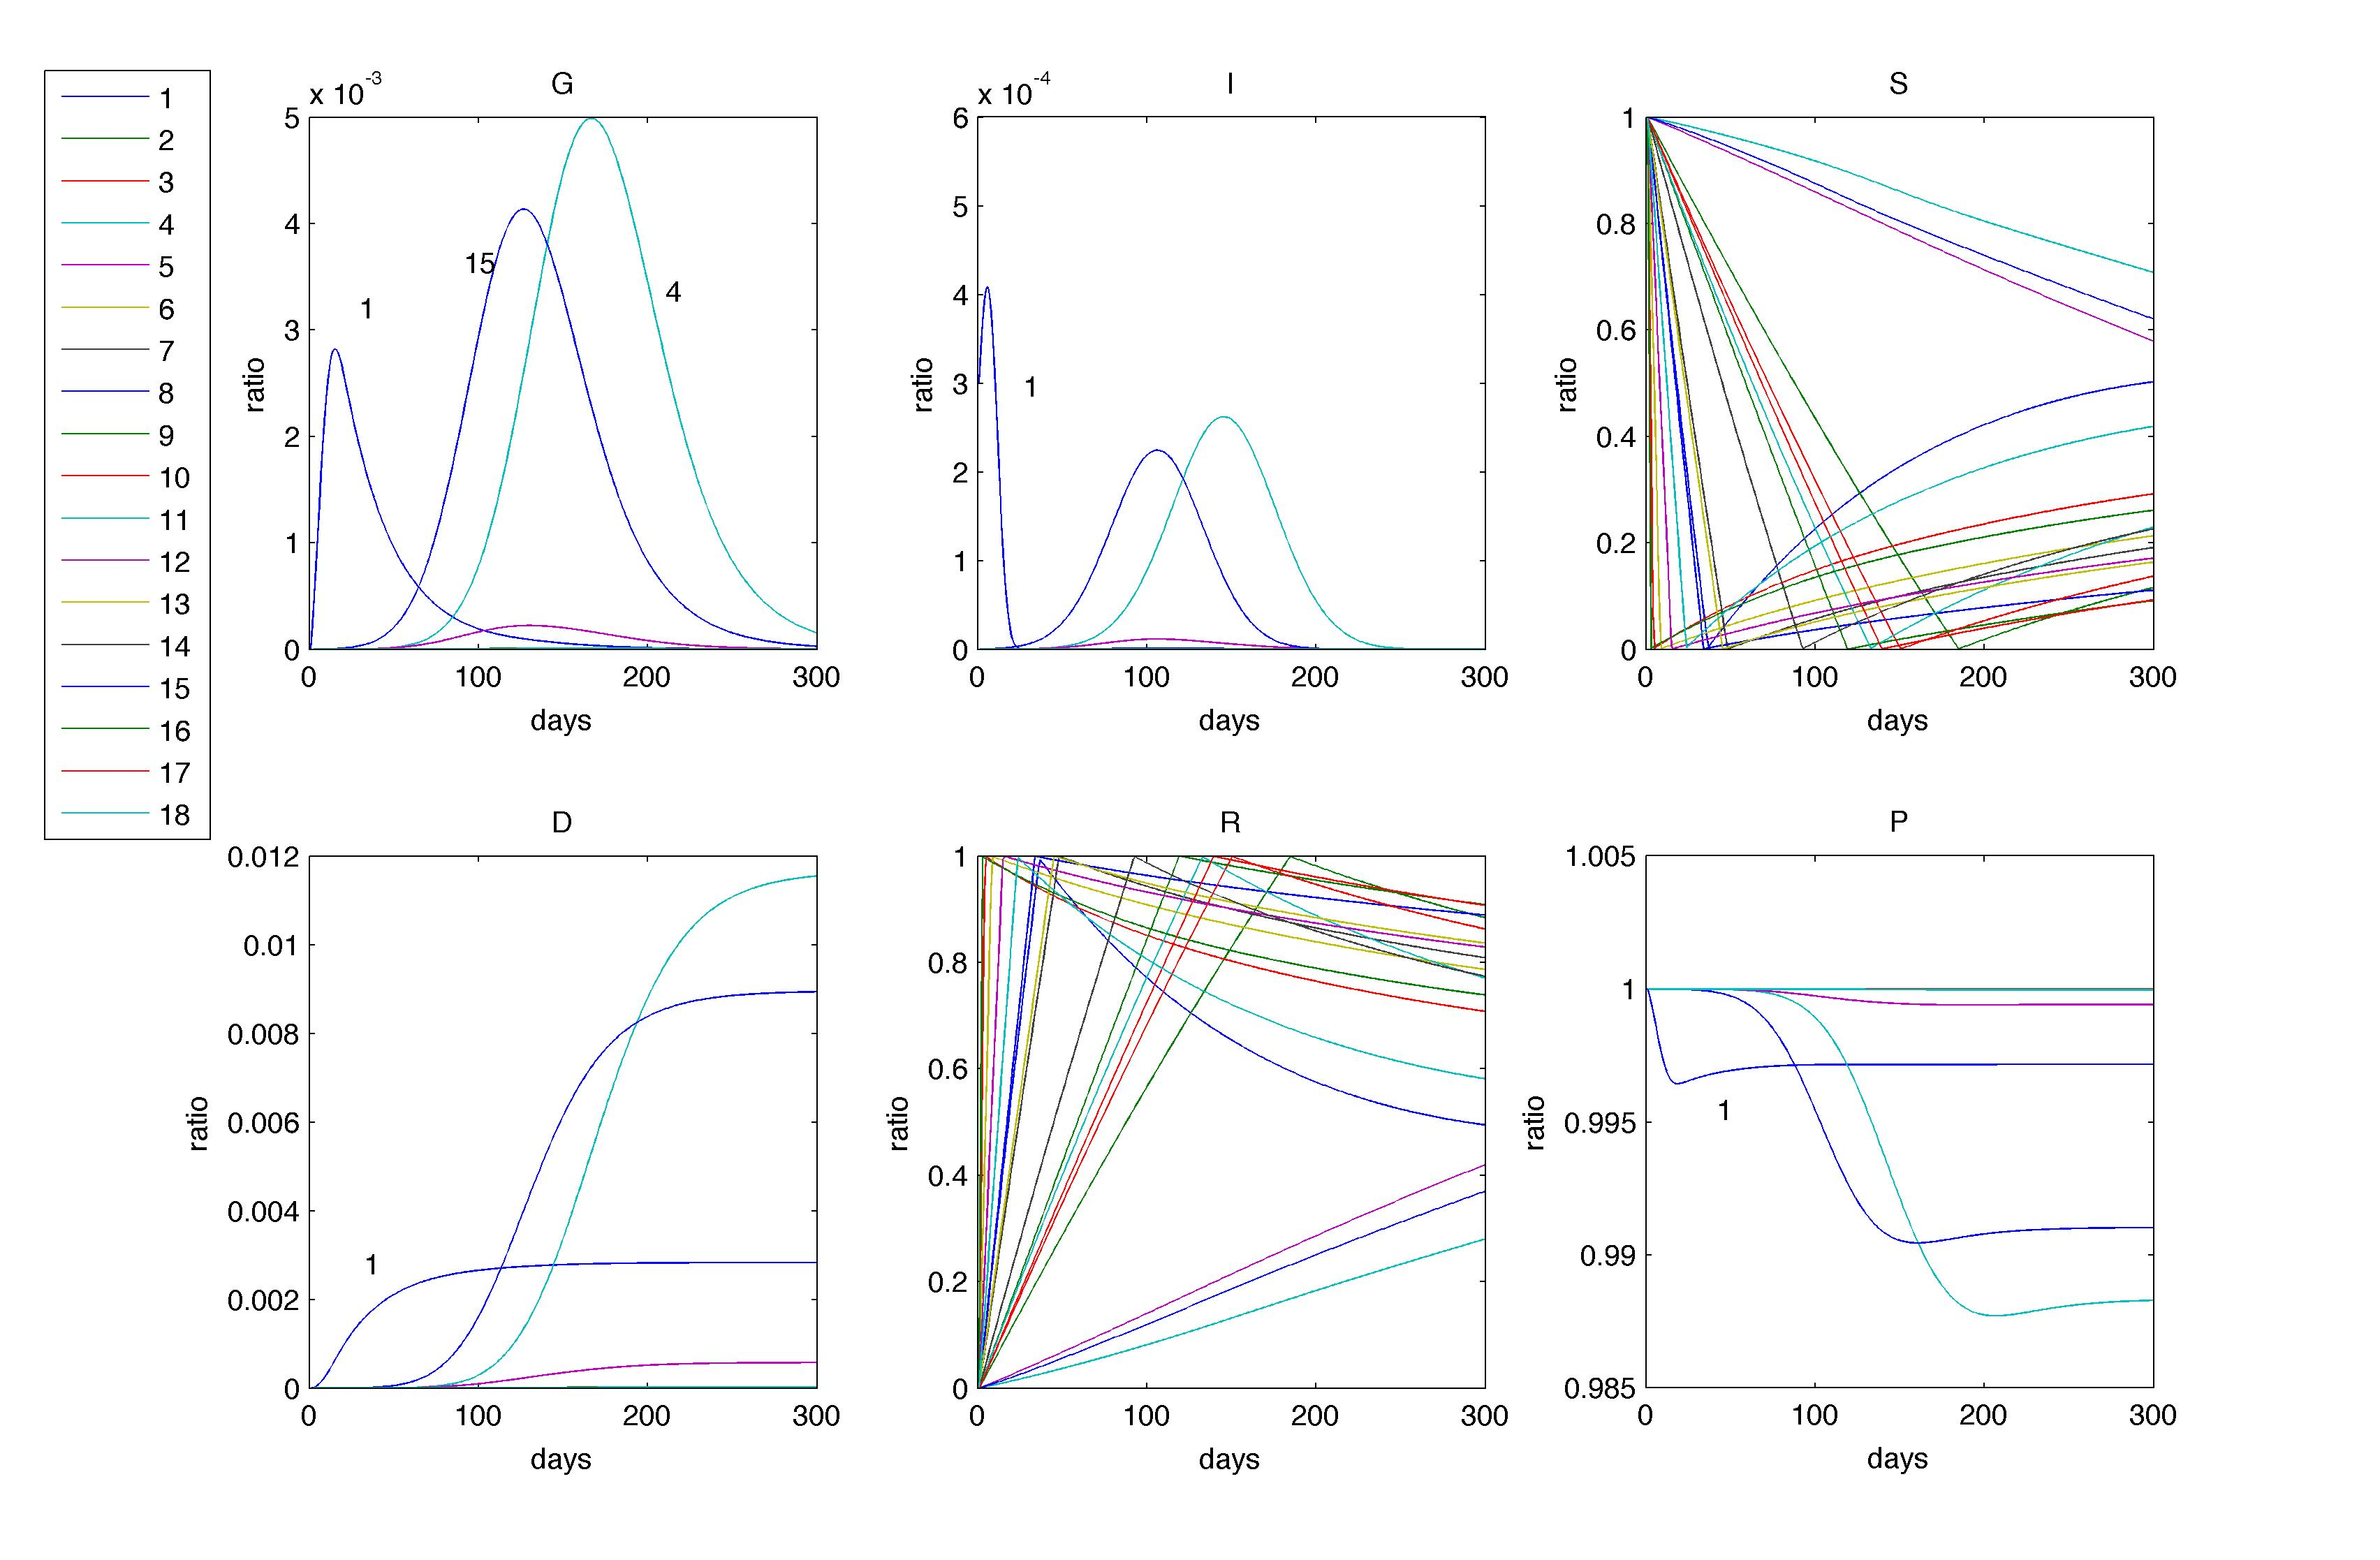
\includegraphics[width = 0.8\textwidth]{multicontrol_1000vacc.jpg}
%\caption{epidemic disease breakout in different cities. $days = 300$, $\alpha = 10^{-4}$ , $drug = 0, vacc = 1000, C = 3, g = 0.8$ and the y axis is the number of people in the group divided by the total number of people in corresponding city. Initially, 10 people are infected in city 1, and all the other people in all the cities are susceptible. The dark blue with label '1' represent city 1. The other dark blue line represents city 15 which is geographically close to city 1. The light green line with label '4' represent city 4 which is the biggest city in the all 18 cities.}
%\label{multicontrol_1000vacc}
%\end{figure}
%
%The observed phenomenon also indicates that some of the cities need more medications than the others. Hence, a carefully organized plan to delivery drugs and vaccines is needed, which will be discussed next.
%
%\subsection{Model for optimizing the medication plan}
%We have seen that different medication plans (the plans to allocate drugs and vaccines) can influence the severity of the spread of disease (measured by the total death due to the disease). Hence, here comes the question: how can we develop a plan that can reduce the number of death as much as possible.
%
%Let us first consider a practical problem where the amount of vaccine that can be provided every day is a constant $vacc_{tot}$ (in the later computation we set the value to $vacc_{tot} = 1800$), and we are required to find out a plan to allocate the vaccines in order that the total death is as small as possible.
%\subsubsection{Genetic algorithm}
%Since there are many degrees of freedom of the possible plans, it is justifiable for us to use optimization algorithm to solve the problem. In order to use genetic algorithm, which is one of the most effective optimization algorithm, it is required that the degree of freedom of the plan which is to be optimized should be encoded into the form of binary `chromosome`. We encoded them into a 180-bit chromosome which is illustrated in figure \ref{chromosome}. The 180-bit chromosome is divided into 18 segments, each of which is representing the amount of vaccines that can be allocated to a city. The length of each segment representing a single city is $chromoUnitLength=10$, which is capable of donating value from 0 to $2^{10}-1$. We may as well donate the value of city $i$ as $w_i$, Hence, we can decide the amount of vaccines each city can get. The number of shares of vaccines that city $i$ can get per day is 
%\begin{equation}
%vacc_i = \dfrac{w_i}{\sum_{j=1}^{18} w_j} vacc_{tot}
%\end{equation}
%
%\begin{figure}
%\centering
%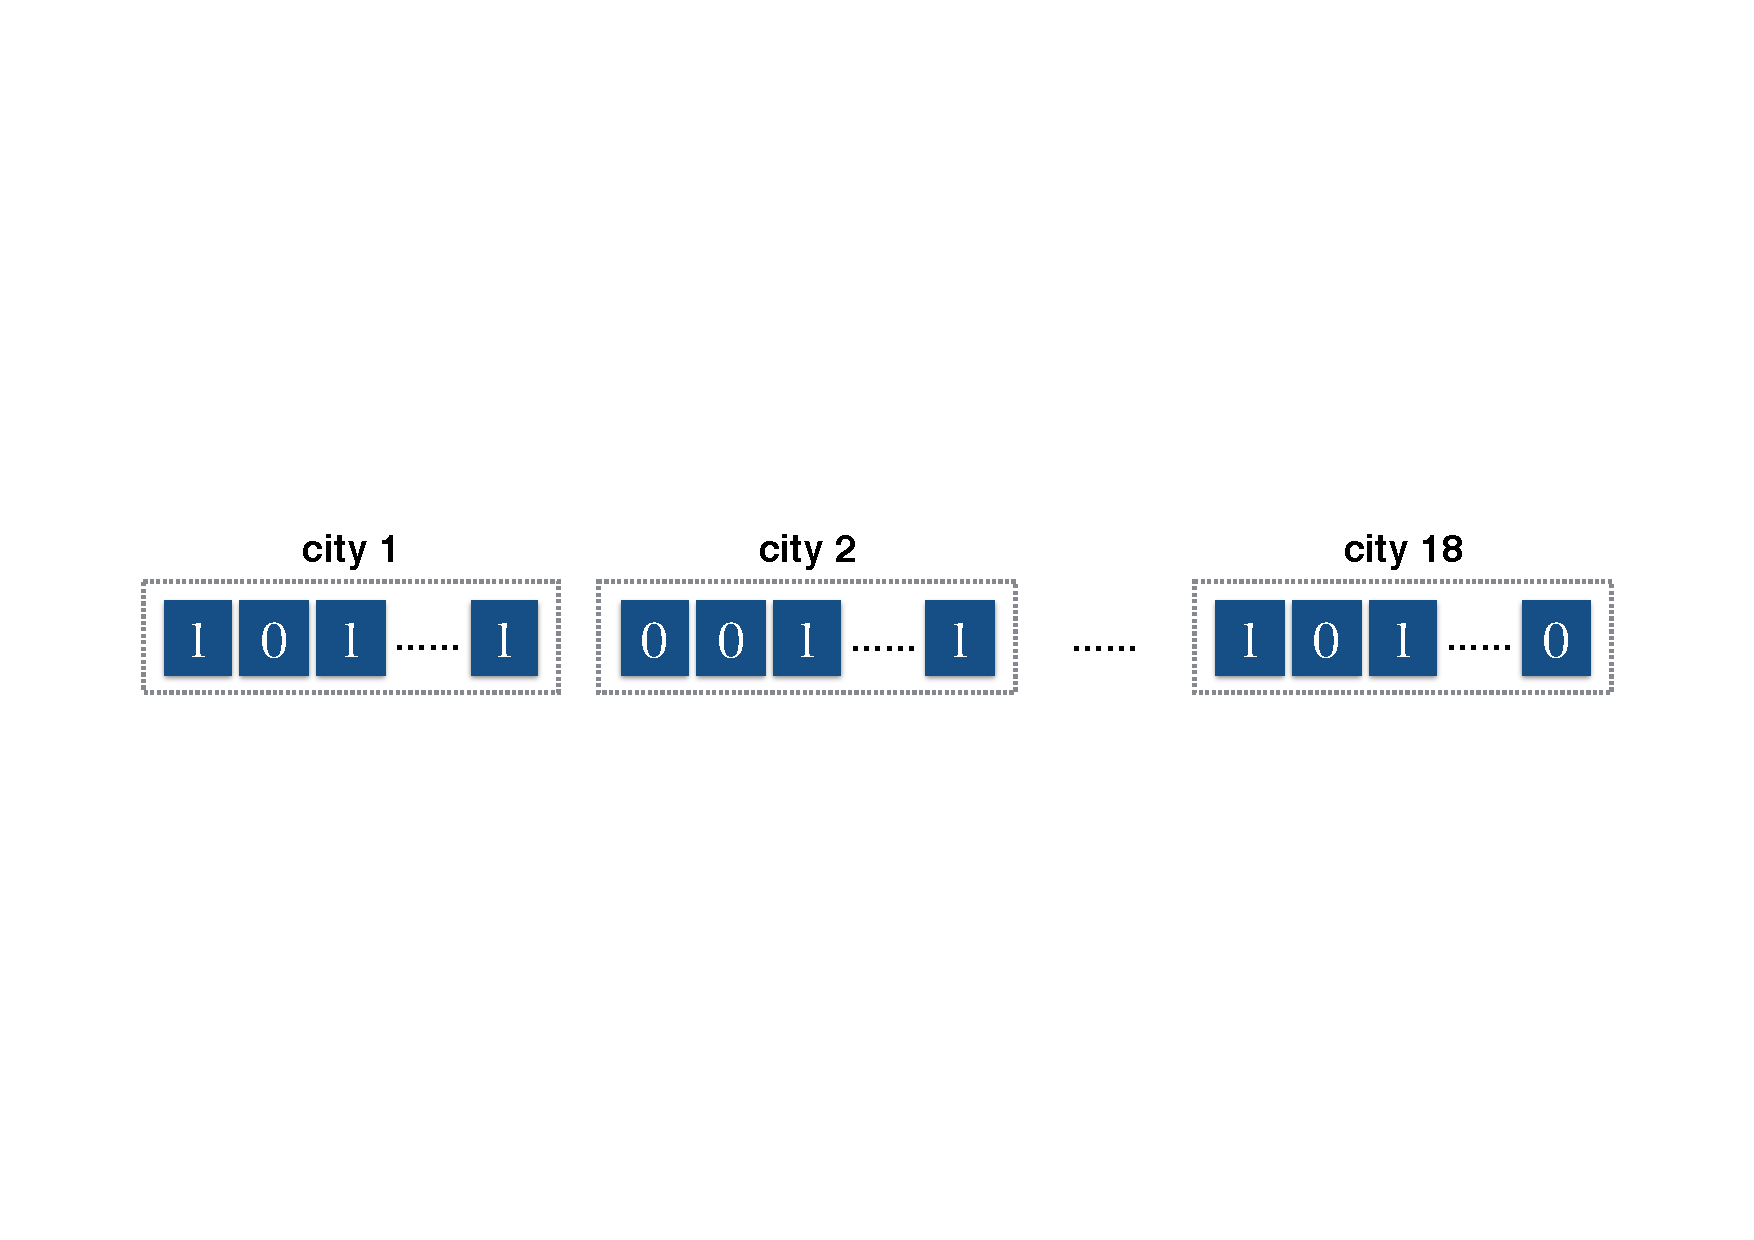
\includegraphics[width = \textwidth]{chromosome.pdf}
%\caption{Encoding}
%\label{chromosome}
%\end{figure}
%
%The process of genetic algorithm we adopted are shown in figure \ref{GA}.
%
%On the stage of initialization (step 1 labeled in the figure), we set the number of generations to be calculated to $generationNum = 1000$, the number of individuals in each generation to $popSize = 200$, the rate of mutation to $mutationRate = 0.01$ and the rate of crossover to $crossoverRate = 0.6$.
%
%On the stage of calculating fitness (step 2), we set the fatality rate as the target function and take it as the value of fitness.
%
%The stage of selecting, crossover and mutation (step 3,4 and 5) are conform the very classic process of genetic algorithm.
%
%\begin{figure}
%\centering
%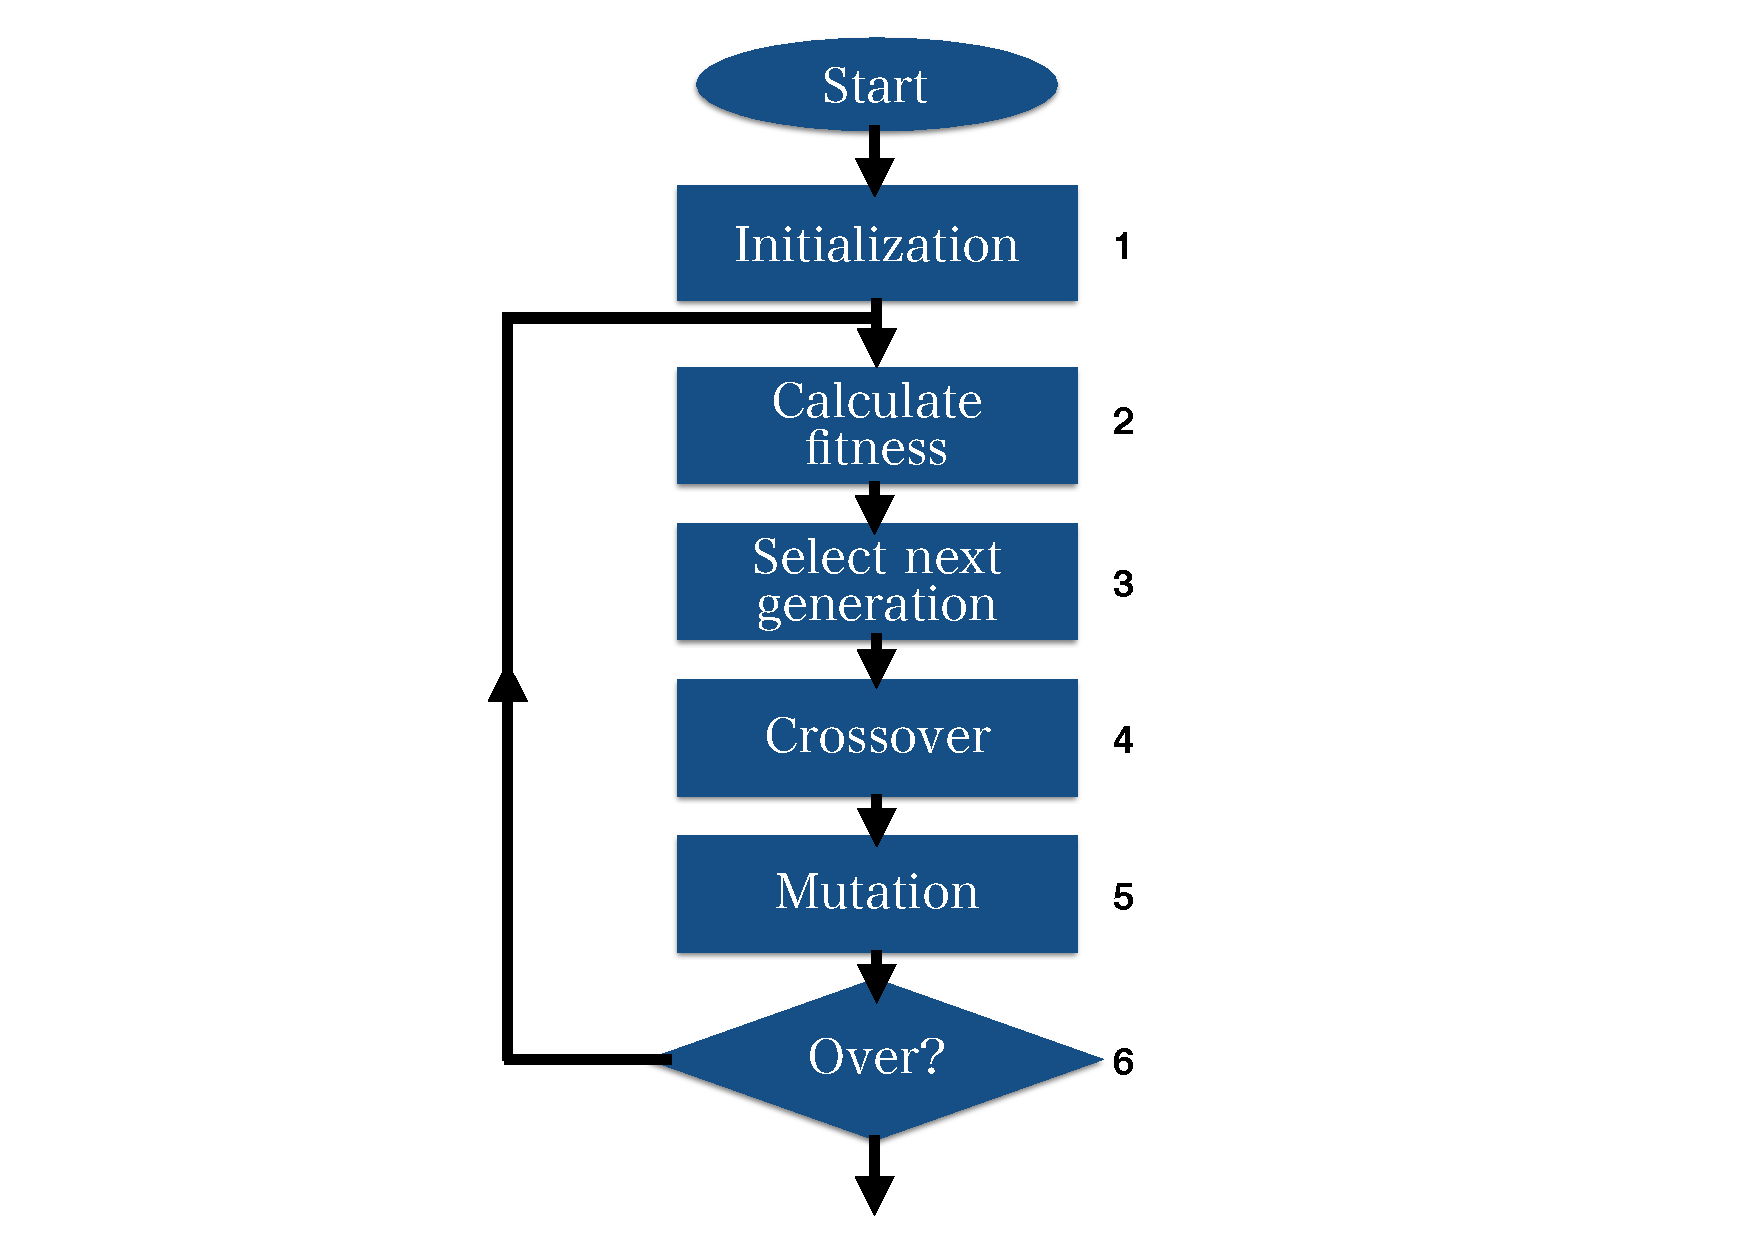
\includegraphics[width = 0.6\textwidth]{GA.pdf}
%\caption{The process of genetic algorithm}
%\label{GA}
%\end{figure}
%
%\subsubsection{Results of computation}
%With parameters shown in table \ref{comppara}. A optimized result is given by our program, which is shown in table \ref{result}. 
%
%The number of death declined from 2768 with randomly generated plan to 380 with the optimized plan shown in table \ref{result}. The declining trend can be easily seen in figure \ref{fitness_avg}.
%
%\begin{table}[]
%\centering
%\begin{tabular}{ccccccccc}
%\hline
%$\beta$ &$k_1$      &$r_s$  &$days$ &$\Delta t$ &$g$    &$C$    &$drug$ & number of initial infected people\\
% 0.32   &0.023      &0.0103 &150    &0.1        &0.8    &3  &0 & 10(in city 1)\\
%\hline
%\end{tabular}
%\begin{tabular}{cccccc}
%\hline
%$vacc_{tot}$&$chromoUnitLegth$ & $generationNum$ &$popSize$  &$mutationRate$ &$crossoverRate$ \\
%1800 &10 &1000            &200        &0.01           &0.6 \\
%\hline
%\end{tabular}
%\caption{Parameters in computation}
%\label{comppara}
%\end{table}
%
%\begin{table}[]
%\centering
%\begin{tabular}{|r|r|r|r|}
%\hline
%label of city&$vacc_i$&population of city & vaccine per capita ($\times 10^{-3}$)\\ \hline
%1&32&33190&0.96983\\ \hline
%2&367&167100&2.1956\\ \hline
%3&3&3222&0.9082\\ \hline
%4&315&1548000&0.20345\\ \hline
%5&185&772900&0.23947\\ \hline
%6&55&7461&7.4029\\ \hline
%7&40&45840&0.86178\\ \hline
%8&14&32660&0.41439\\ \hline
%9&31&114000&0.26952\\ \hline
%10&98&137700&0.71456\\ \hline
%11&41&117100&0.34673\\ \hline
%12&94&13990&6.7195\\ \hline
%13&24&43100&0.55164\\ \hline
%14&48&85020&0.5679\\ \hline
%15&329&1011000&0.32562\\ \hline
%16&51&1870&27.1889\\ \hline
%17&27&132700&0.20398\\ \hline
%18&47&21960&2.132\\ \hline
%\end{tabular}
%\caption{A optimized plan for allocating vaccine with $vacc_{tot} = 1800$ }
%\label{result}
%\end{table}
%
%\begin{figure}
%\centering
%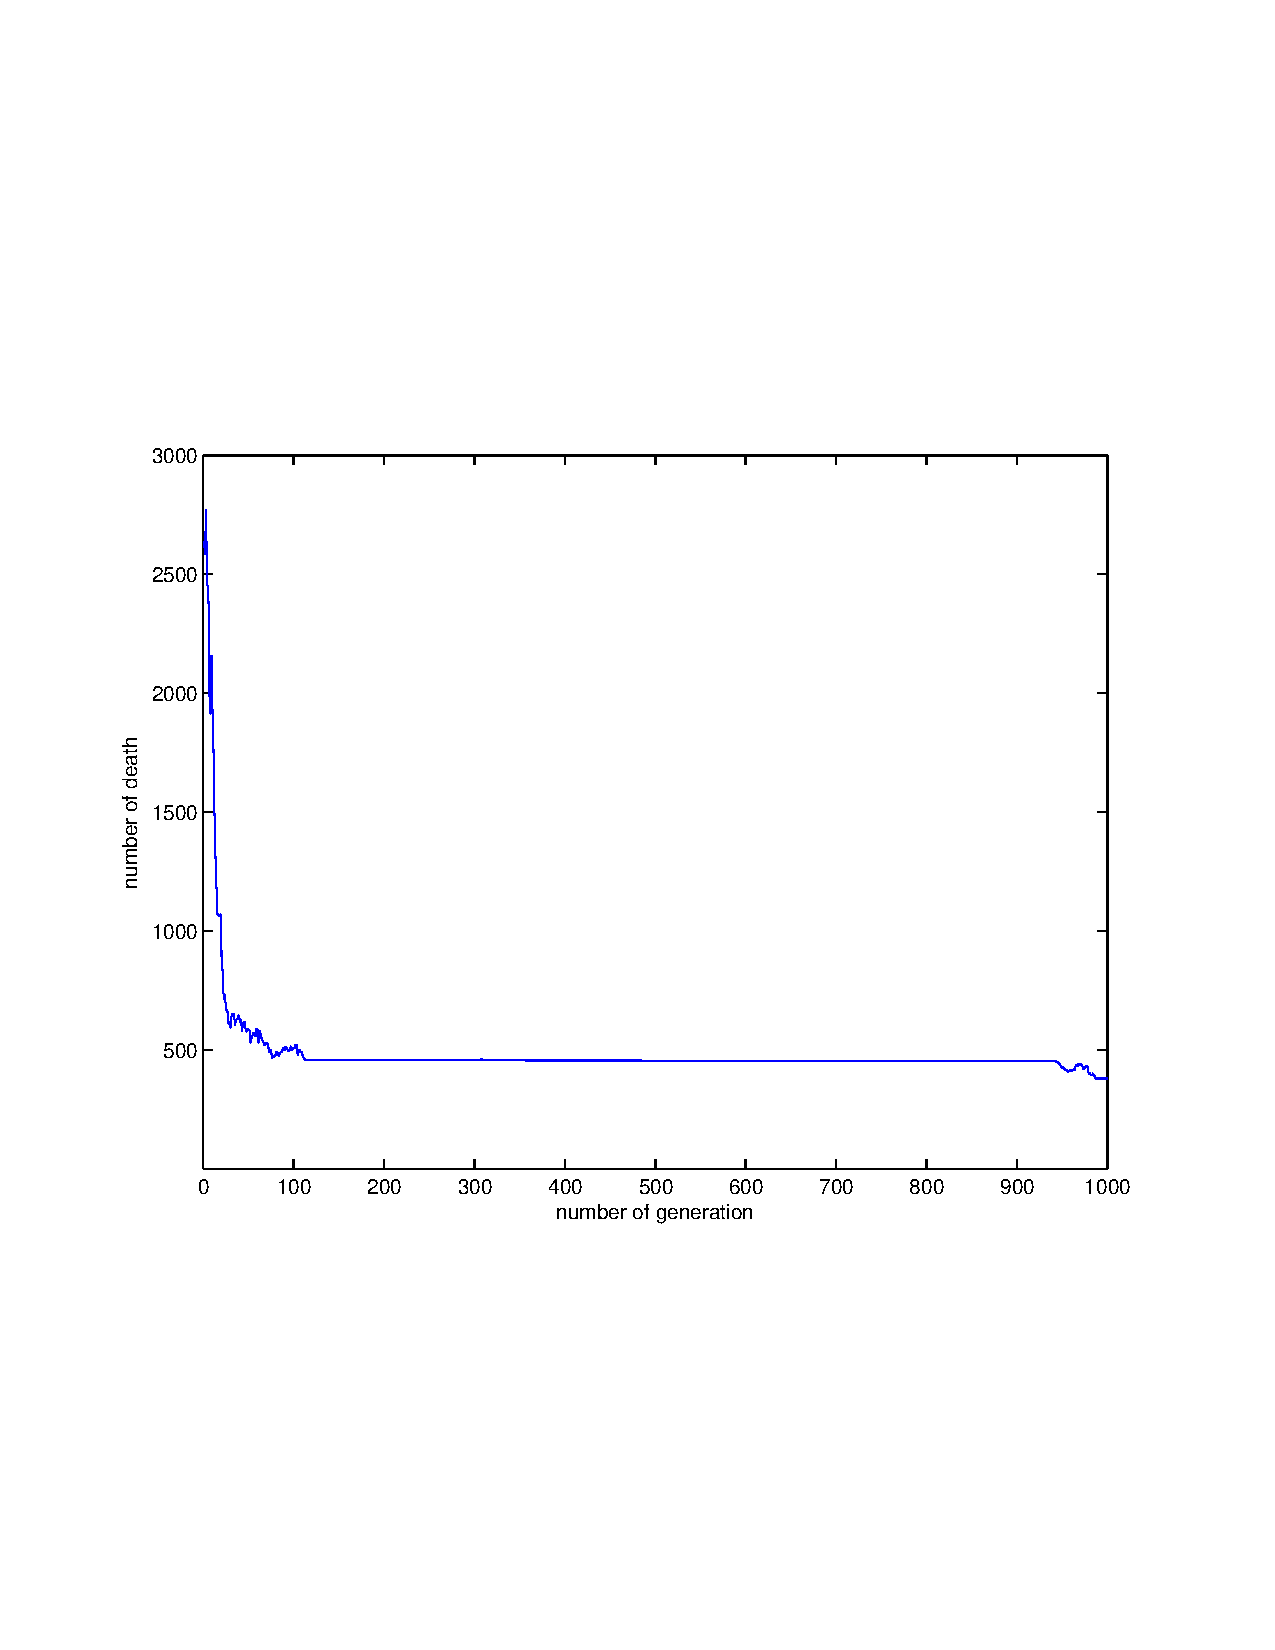
\includegraphics[width = 0.6\textwidth]{fitness_avg.pdf}
%\caption{The number of death declines with the optimization of the plan. The x axis is for the number of generations of genetic algorithm and the y axis is for the number of death in all the 18 cities.}
%\label{fitness_avg}
%\end{figure}
%
%\subsubsection{Analysis of the result}
%The result is analyzed from following aspects.
%\begin{enumerate}
%\item The two biggest cities - city 4 and city 15 - are allocated for more than 300 shares of vaccines, which is remarkably more than others. This outcome is easy to understand. The more people in the city, the more shares of vaccine are needed.
%\item Some of cities are allocated more shares of vaccine compared with their population, where city 16 is a significant example. City 16 is a small town, but it has the largest amount of vaccine per capita. It is easy to understand considering the geographic location of city 16. City 16 lies in the center of the cities we selected, which plays a significant role in the transmission of pathogen from one city to another. Once huge amount of vaccine is delivered to this city, the route of transmission of pathogen is greatly cut off.
%
%That the city near the center of network needs more vaccine per capita is clearly shown in figure \ref{vaccine_per_capita.pdf}.
%\item The largest amount of vaccine is allocated to city 2, which is a relatively big city and locates relatively in the center of all the cities, confirming the previous inference.
%\item Since people flow is supposed to be determined by the distances between cities, the amount of vaccine per capita is related to geographic location of cities. In real practice, the people flow is determined by more factors, such as convenience of traffic, so it is not difficult to imagine that \textbf{the cities that lie in the center of people flow network need larger amount of vaccine and drug per capita}.
%\item The computation above is varying the delivery plan for vaccine when the plan for drug is invariant. When the delivery plan for vaccine is invariant, the optimized delivery plan for drug has similar characteristics. Hence, we just list the mere optimized plan for drug in table \ref{drug} and are not repeating the similar interpretation.
%\end{enumerate}
%
%\begin{figure}
%\centering
%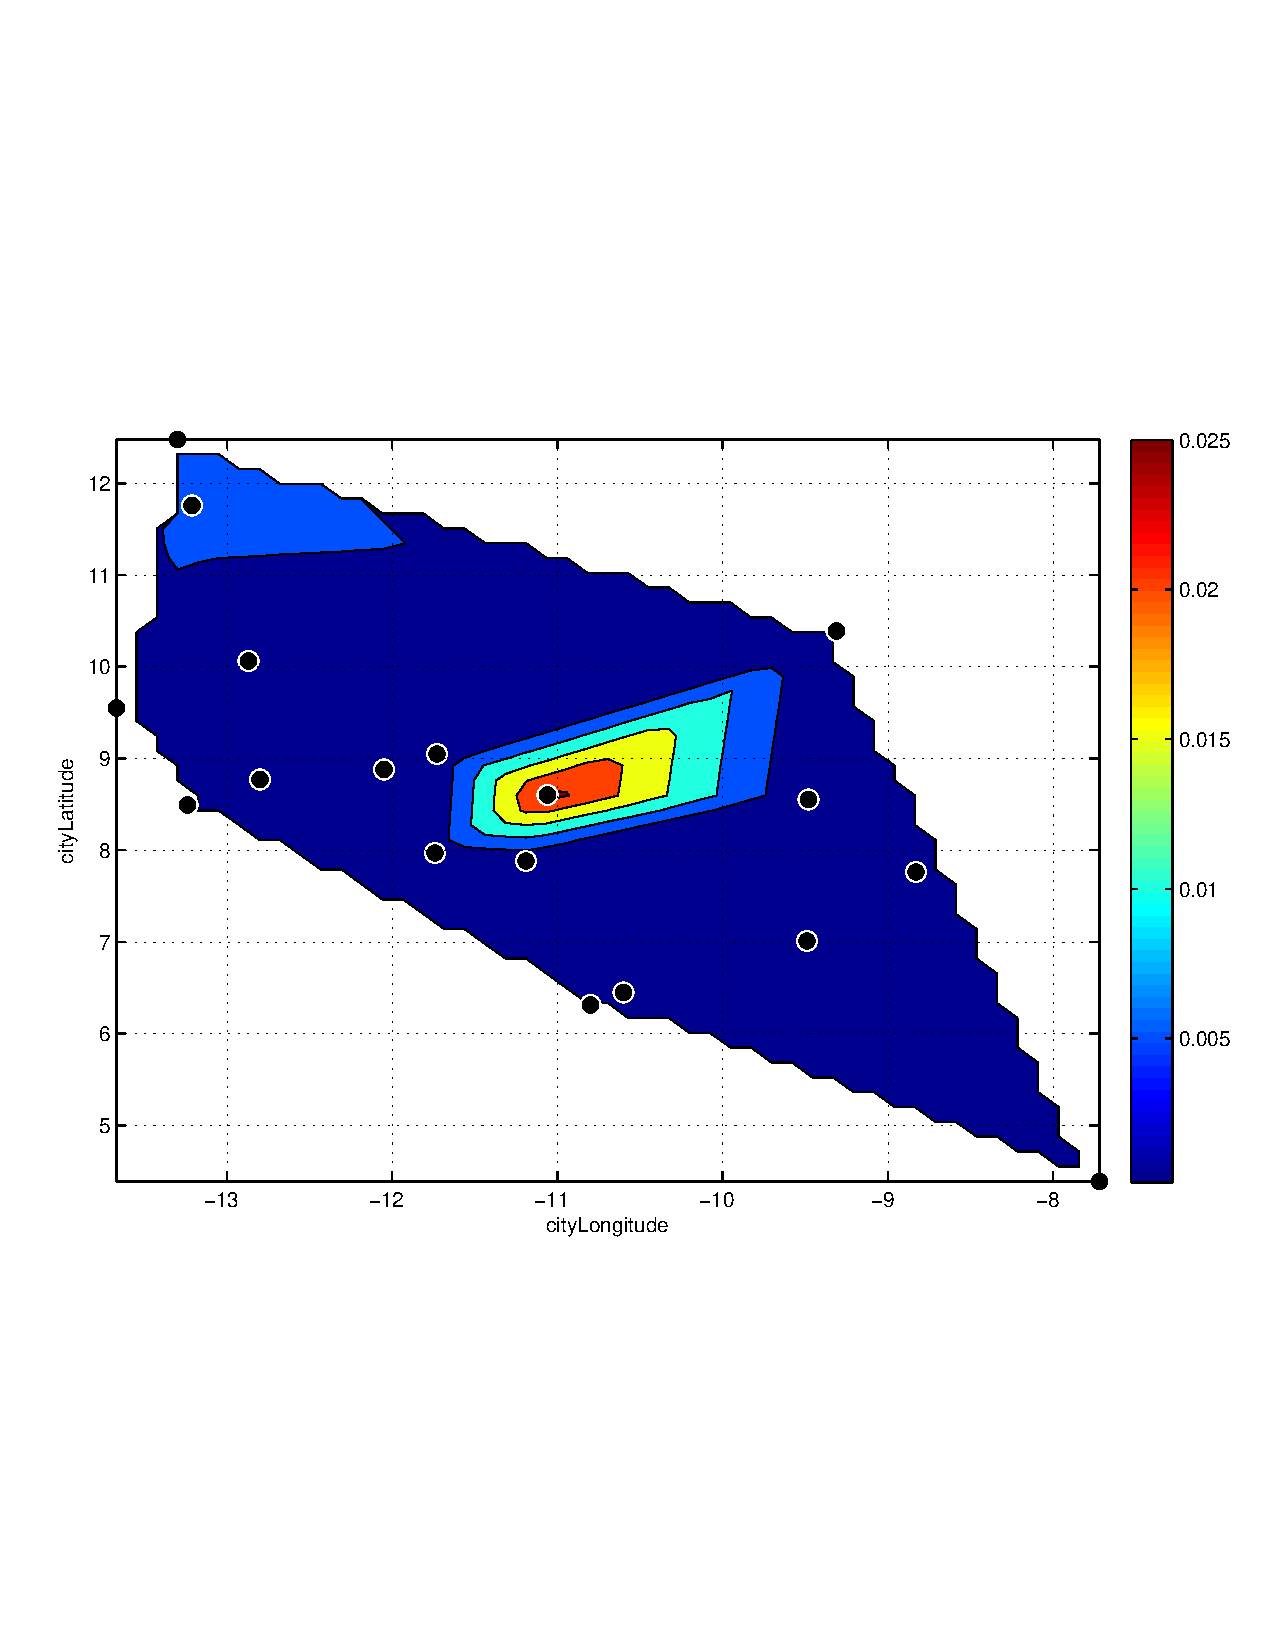
\includegraphics[width=0.6\textwidth]{vaccine_per_capita.pdf}
%\caption{The contour plot of vaccine per capita. The black spots represent locations of the 18 cities.}
%\label{vaccine_per_capita.pdf}
%\end{figure}
%
%\begin{table}[]
%\centering
%\begin{tabular}{|r|r|r|r|}
%\hline
%label of city&$drug_i$&population of city & drug per capita ($\times 10^{-3}$)\\ \hline
%1&32&33190&0.9497\\ \hline
%2&111&167100&0.6643\\ \hline
%3&113&3222&34.9531\\ \hline
%4&93&1548000&0.060143\\ \hline
%5&112&772900&0.14476\\ \hline
%6&76&7461&10.1765\\ \hline
%7&59&45840&1.2819\\ \hline
%8&37&32660&1.1336\\ \hline
%9&14&114000&0.12545\\ \hline
%10&107&137700&0.78005\\ \hline
%11&31&117100&0.26779\\ \hline
%12&1&13990&0.077239\\ \hline
%13&6&43100&0.1433\\ \hline
%14&57&85020&0.67318\\ \hline
%15&108&1011000&0.10657\\ \hline
%16&22&1870&11.6608\\ \hline
%17&9&132700&0.067749\\ \hline
%18&12&21960&0.54899\\ \hline
%\end{tabular}
%\caption{A optimized plan for allocating drug with $drug_{tot} = 1800$ }
%\label{drug}
%\end{table}

\section{Problem 1: Design for Decision Model}
%\subsection{Strengths}
\begin{enumerate}
\item \textbf{Our model is simple and easy to understand} \\
Our model is the simplest model we can conceive to reflect the impact of concerned independent variables (factors regarding medication) and to solve the problem lifted by the question. 

Our single-city model is based on the most elegant model in the field of epidemiology - the SIR model, and we reconstruct the model (mainly add two clusters of people) in order to introduce concerned independent variable into our system. 

Our multi-city model is based on our single-city model and introduce only one `people flow` to obtain the geographic characteristic of the spread of disease.

\item \textbf{Our model is effective and in good agreement with the reality} \\
Simple as they are, they are effective in reflecting the complex relationships between numerous variables and parameters, and they not only reveal the intrinsic characteristics of the spread of disease itself but also successfully link factors of medication to the spread of disease.

Comparing with the data we have find from several resources, the results of our model not only correspond the general trend of the records but also resemble the reality in some critical features.

\item \textbf{Good extensibility} \\
Flow of people is a critical factor determining the spread of disease. Although our multi-city model only set the volume of people flow as a function of mere geographic distribution and population of cities, the determinants of people flow can be adjusted when other possible factors are considered. Then, the adjusted model can be applied to study the impact of other possible factors relating to epidemiology.

\end{enumerate}



%\subsection{Weaknesses}
\begin{enumerate}
\item \textbf{Our model is just a rough model} \\
For simplicity, we have neglected many potential parameters, variables or processes, and have made numerous assumptions. Eg. we did not consider the relationship between separate individuals and we did not dig deeper into the properties of social network which is a quite essential part determining the spread of disease. Some important general or specific factors are also neglected by us, a interesting example of which is a folk custom prevalent in the studied region that relatives kiss the death, which plays a significant role in the spread of disease and is categorized into \emph{Super Spread Event}(SSE) academically. 

\item \textbf{Our model is only a continuous model} \\
Numbers of people, number of shares of drug/vaccine, etc. are important quantities in all the process of modeling and computation. For simplicity, we regard the numbers as directly real numbers instead of integers. It is justifiable when the numbers are large, since the decimal part of the number is negligible; when the system scales down, however, the statistics dose not work and the outcome deviates a lot from reality.
\end{enumerate}
\section{Problem 2: Decisions for Drivers and Analysis for the Decision Model}
\subsection{Data Preparing}
\begin{enumerate}
\item \textbf{Raw Data} \\
The overview of taxi data and flight data is shown in the form of data distribution statistics chart as followed.And the detailed datas are placed in appendix.
\begin{figure}[H]
\centering
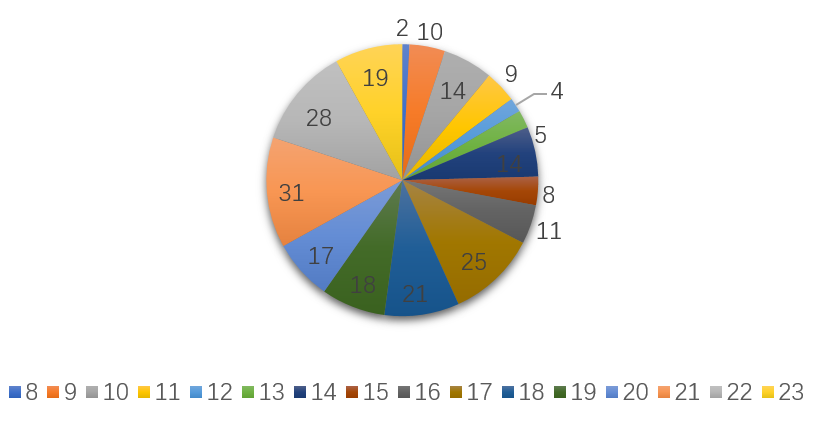
\includegraphics[width=0.7\textwidth]{figures/Q2_1.png}
\caption{Flight data of Pudong Airport 20180602 obtained by crawling}
\label{fig:label}
\end{figure}

\begin{figure}[H]
\centering  
\subfigure[Passenger distance distribution of taxi in Shanghai in 2015]{
\label{Fig.sub.q2111}
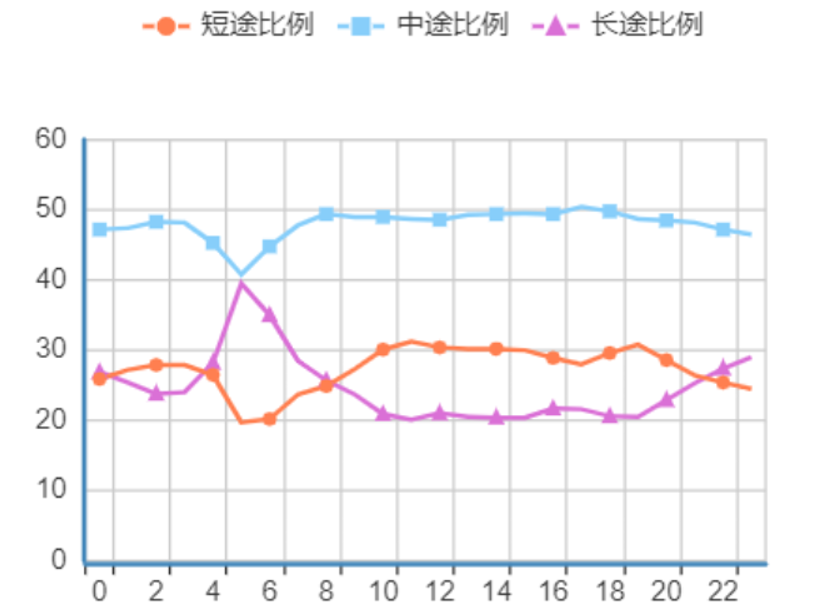
\includegraphics[width=0.45\textwidth,height = 4cm]{figures/Q2_2.png}}
\subfigure[Average speed distribution of taxis in Shanghai in 2015]{
\label{Fig.sub.q2112}
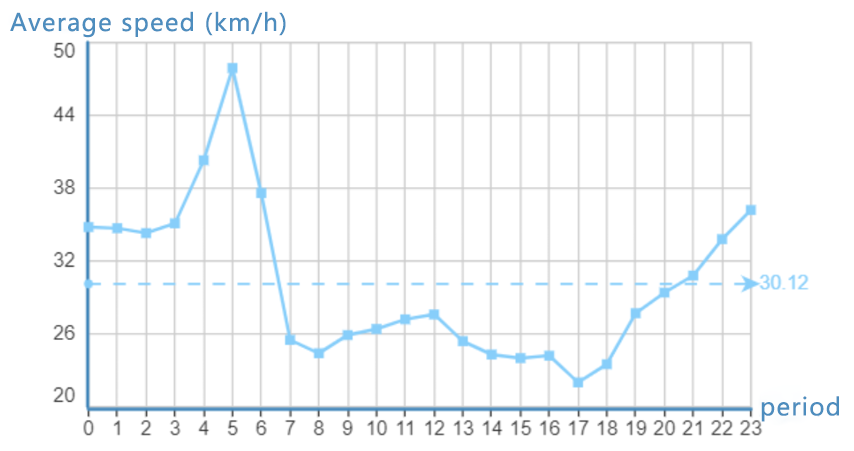
\includegraphics[width=0.45\textwidth,height = 4cm]{figures/Q2_3.png}}
\caption{ Taxi Data }
\label{Fig.q211}
\end{figure}

\item \textbf{Processed Data} \\

\begin{figure}[H]
\centering
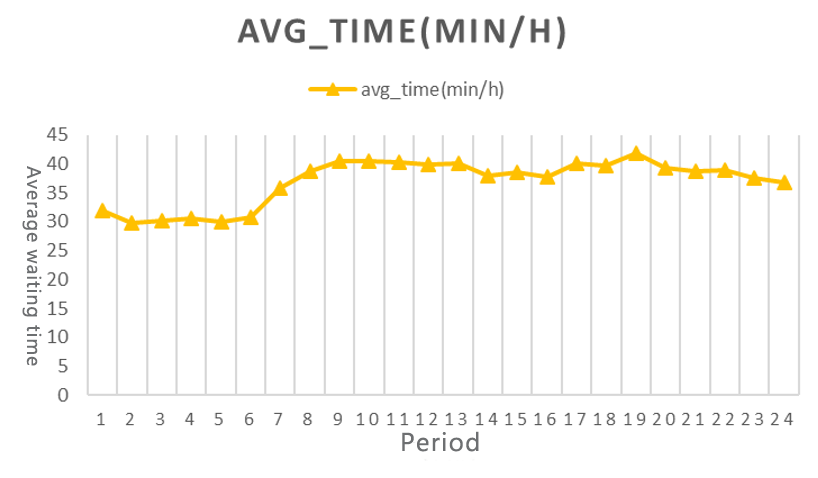
\includegraphics[width=0.7\textwidth]{figures/Q2_4.png}
\caption{Average waiting time of receiving orders in urban areas in different time periods}
\label{fig:label}
\end{figure}
From the raw data, we do a lot of processing, and finally extract 2077 pieces of data as clustering candidate data.And the field is shown in below table.And we put forward some assumptions: If the taxi enters Pudong Airport in empty state at $t_{empty}$ and becomes loaded at $t_{busy}$, the starting time of queuing is assumed to be $t_{empty}$. If the taxi enters the airport in loaded state and becomes empty at $t_{empty}$ and becomes loaded at  $t_{busy}$ again, the starting time of queuing is assumed to be $t_{empty}$.
\begin{table}[H]
\centering
\caption{Candidate data for clustering}
\begin{tabular}{|l|p{5cm}|p{7cm}|}
\hline
\textbf{Field} & \textbf{Description} & \textbf{Calculate Method} \\ \hline
$Id$ & taxi number & from origin data \\ \hline
$Time$ &  the time begin queuing at Pudong Airport & from origin data  \\\hline
$Wait\_time$ & taxi queuing time in airport & $t_{busy} - t_{empty}$  \\ \hline
$taxi\_density$ & Accumulated number of taxis in Pudong airport within 2 hours ahead of $Time$ & Use a set to record all the unique taxi number in these two hours, and the size of the set is the taxi density.\\ \hline
$flight\_density$ & Total number of passengers landing at Pudong airport within 2 hours ahead of $Time$ & Sum of the total number of passengers of the flight with the planned landing time in these two hours\\ \hline
\end{tabular}
\end{table}
\end{enumerate}



\subsection{Parameter Calibration}

\begin{table}[H]
\centering
\caption{ Parameter Setting for Model}
\begin{tabularx}{15cm}{llX}  % 10cm 減去前兩個欄位寬度後,剩下的通通給
\hline                      % 第三欄位使用,文字超出的部份會自動折行
Symbol & Value  & Meaning  \\
\hline
${L}_1$  & 46.4 & Unit: km, the approximate distance from Pudong Airport To Downtown\\
${t}_DE$ & 0.576014 & Unit: H, the average waiting time of passengers in the queue in this period, selected from the clustering result set, time point is 19:17 \\
$\alpha$  & 1 & Weather factor, for the convenience of calculation, it is assumed that the weather is in good condition\\
${V}_2$ & $f(t)$ &Unit: km/h, average speed in urban area,$f(t)$ is the function to calculate ${V}_2$ \\
${V}_1$   & 64.7 & Unit: km/h, average speed from Pudong to downtown\\
$\beta$  & 1 & Road condition factor, also assuming good road condition\\
$o$  & 0.088 & Unit: L/km, fuel consumption per mileage\\
$k$  & 7.13 & Unit: \textyen/L, unit oil price\\
${f}_1$  & 14 & Unit: \textyen, starting price of taxi in Shanghai\\
$a$  & 3 & Unit: km, first gradient mileage limit\\
${f}_2$  & 2.5 & Unit: \textyen, more than 2.5 \textyen/km over $a$\\
$b$  & 15 & Unit: km, first gradient mileage limit\\
${f}_3$  & 3.6 & Unit: \textyen, over part B, 3.6 \textyen/km\\
$\mu$  & 0.15 & Weighting factors for time periods\\
\hline
\end{tabularx}
\end{table}


\subsection{Model Calculation}

After standardizing the candidate data, 1000 pieces of 2077 pieces of data are randomly selected as samples. Each sample is $(time, flight\_density, taxi\_density, wait\_time)$, which corresponds to the parameter $(T,{N}_a,{N}_c,{t}_q)$ in Task 1, we set $k = 4,5,6,7$ for K prototype clustering, and bring $k$  into the following formula:
\[E = \sum_{i=1}^{k} \sum_{i=1}^{n} {D}_s({X}_i,{X}_{center})\]
Calculating the mean square error of each cluster set under each $k$ value:
\begin{table}[H]
\caption{Mean Square Deviation}
\begin{center}
\begin{tabularx}{5cm}{p{2cm}|p{3cm}}
\hline
K & E  \\
\hline
4 & 100.56  \\
5 & 35.94 \\
6 & 165.67  \\
7 & 189.86 \\
\hline
\end{tabularx}
\end{center}
\end{table}
It can be concluded from above table that the clustering effect is  best when $k = 5$, and the clustering diagram after clustering is as follows:
\begin{figure}[H]
\centering
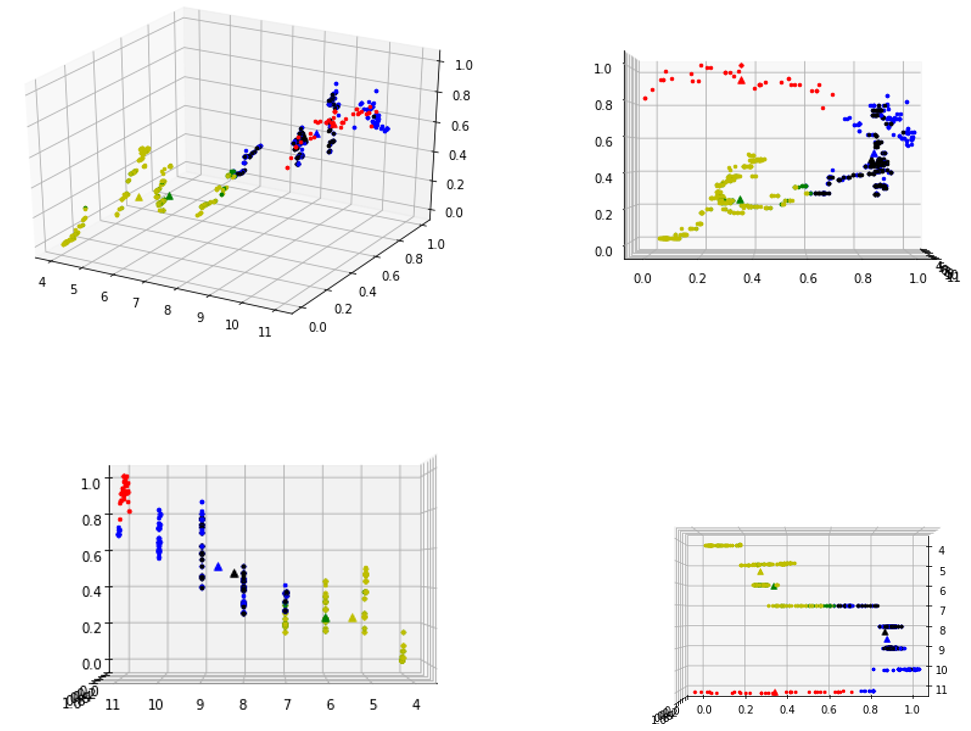
\includegraphics[width=0.7\textwidth]{figures/Q2_5.png}
\caption{Distribution of Clustering Results}
\label{fig:label}
\end{figure}
When $k = 5$, cluster sets and cluster centers are saved for the following calculation. Then, 50 pieces of data are randomly selected from 2077 pieces of data as decision samples (excluding the $wait\_time$ field, and the data is in the appendix), and brought into model. The net profit of each sample in the queue and the net profit returned to the urban area are calculated. The overall comparison chart is as follows:

\begin{figure}[H]
\centering  
\subfigure[Net income per unit time - Number of passengers]{
\label{Fig.sub.q2111}
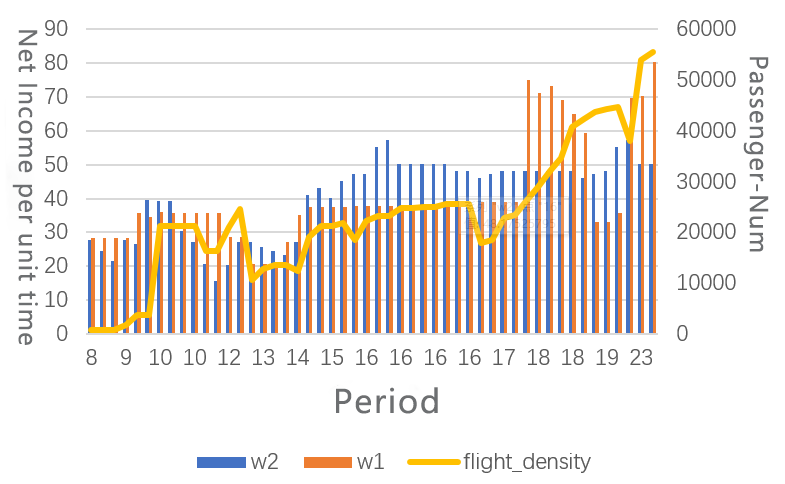
\includegraphics[width=0.45\textwidth,height = 5cm]{figures/Q2_6.png}}
\subfigure[Net income per unit time -Number of taxis]{
\label{Fig.sub.q2112}
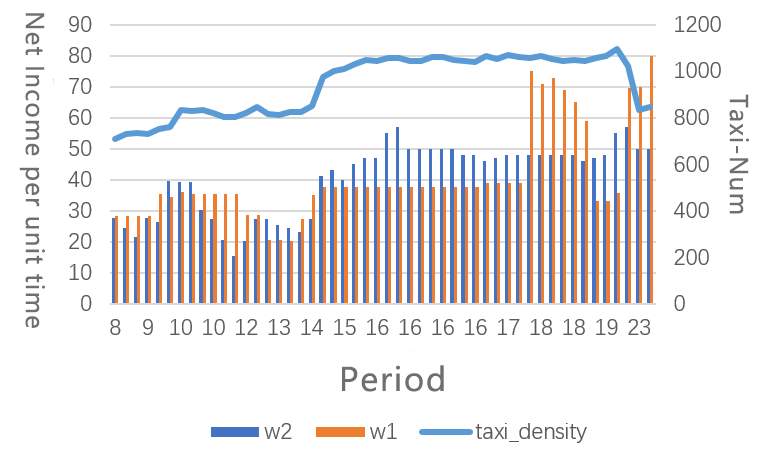
\includegraphics[width=0.45\textwidth,height = 5cm]{figures/Q2_7.png}}
\caption{Comparison of overall results}
\label{Fig.q211}
\end{figure}
According to the above figures, we can see the decision scheme made by the model:
\begin{table}[H]
\centering
\caption{ Decision Plan}
\begin{tabularx}{15cm}{lX}  
\hline                      
Decision & Period   \\
\hline
Queue up  & $8:00-9:00 \;\&\; 11:00-12:30 \;\&\; 18:00-19:00 \;\&\; 22:00-24:00$\\
Return to urban & $9:00-11:00 \;\&\; 12:30-18:00 \;\&\; 19:00-22:00$\\
\hline
\end{tabularx}
\end{table}
This plan is the choice we give to taxi drivers in this airport.

\subsection{Rationality Analysis}
The decision calculated by our model has the following characteristics:

\begin{enumerate}
\item Tend to choose a later night (such as 22:00-24:00), which is consistent with the actual situation of life. Because the choice of public transport at night becomes scarce, the probability of flight passengers choosing to take taxis will increase. Just as the proportion of night flight passengers choosing taxis in Pudong Airport calculated by China Daily is as high as 45\%, in this case, the demand for taxis will be large, and the waiting time of drivers will be shortened. In addition, the charge of night taxi is higher, especially in the airport where the order receiving rate is probably long-distance, the driver's income will increase significantly. Therefore, drivers will naturally prefer to wait in line for passengers in this period of time.
\item Tend to make the choice of waiting in line at the peak of urban traffic (18:00-19:00 \& 8:00-9:00). In fact, it is also easy to understand that when the urban area is in the rush hour of going to and from work, the road is blocked and the average traffic jam time is long, which will lead to the decrease of the driver pick-up frequency, the increase of the air run time and the increase of the fuel consumption, so the taxi drivers are more inclined to avoid such peak periods.
\item Tend to make the choice of waiting in line when the passenger demand is small (11:00-12:30). In the period of noon, according to people's normal life, they are at the time of lunch. At this time, the demand for taxis in the urban area is bound to be small.
\item  In other time periods (mostly during the day), the proportion of airport passengers who choose to take taxis is small (only 15\% of Pudong Airport passengers choose to take taxis during the day according to China Daily net). If they queue up, they will waste a lot of time. On the contrary, in the urban area, the road traffic condition is normal, which is more conducive to business.
\end{enumerate}
And about rationality analysis
\begin{enumerate}
\item The parameters such as taxi time interval, average speed distribution, average waiting time for single receipt and taxi pricing are all open real data. At the same time, the extracted airport taxi sample data is obtained through a large number of screening statistics, which is consistent with the actual situation.
\item The clustering model used to calculate the waiting time of the queue has a better clustering effect. After the evaluation of the contour coefficient combining the two factors of cohesion and separation, that is, for each vector in K clusters, the contour coefficient\cite{kaggleCompetition} of each vector is calculated by the following formula:
\begin{equation} S(i) = \frac{b(i)-a(i)}{max(a(i),b(i))}\end{equation}
\end{enumerate}

\subsection{Dependency Analysis}
Our decision model consists of six variables: $N_a$,$N_c$,$L_2$,$V_2$,$t_w$,$T$,and we calculate the average and the maximum, minimum values of them respectively so as to conduct sensitivity analysis. And the values are shown in below table.
\begin{table}[H]
\centering
\caption{Parameter sensitivity analysis}
\begin{tabularx}{15cm}{c|c|c|c|c} 
\hline                    
Parameter & Max & Min & Avg & Description\\
\hline
$N_a$  & 55923 & 740 & 23187 & flight density\\
$N_c$  & 1107 & 703 & 943 & taxi density \\
$L_2$  & 15.5647 & 12.0199 & 12.9387 & taxi carrying distance per order\\
$V_2$  & 47.9 & 22.0 & 30.1375 & taxi average speed in various time\\
$t_w$  & 0.982 & 0.4974 & 0.6155 & average waiting time for receiving orders \\
$T$  & 23 & 8 & 11 & time(in 24 hours)\\
\hline
\end{tabularx}
\end{table}

Set the i parameter $C_i$ of every parameter in $(N_a.N_c,L_2,V_2,t_w)$from its minimum value to the max value with stride $s$:
\begin{equation} s = \frac{C_{i\_max}-C_{i\_min}}{10}\end{equation}
That is $\{C_{i\_min},C\_{i_min}+s,C_{i\_min}+2s,\cdots,C_{i\_max}\}$,and the remaining five parameters are set to average value.Then bring these variables into the decision model, so that we can get $\{d_{w\_i\_1},d_{w\_i\_2},\cdots,d_{w\_i\_10}\}$ where ${d_{w\_i\_k} = w_{1\_i\_k} - w_{2\_i\_k}}$.,So that the ratio of the increment of each $d\_w$ relative to the former to the increment of $C\_i$ can be obtained, that is:
\begin{equation} r_{w\_i\_k+1} = \frac{|\frac{d_{w\_i\_k+1} -d_{w\_i\_k} }{d_{w\_i\_k}}|}{\frac{s}{C_{i\_min}+ks}}\end{equation}
we can get $r_{w\_i} = [0,r_{w\_i\_2},r_{w\_i_3},r_{w\_i\_4},r_{w\_i\_5}]$.By calculating each of the six parameters, a sensitivity matrix of the six parameters can be obtained:
\begin{equation}
r_{w} = 
\left[
\begin{matrix}
 r_{w\_1\_1}  & \cdots & r_{w\_1\_10}      \\
 \vdots  & \ddots & \vdots \\
  r_{w\_6\_1}     & \cdots & r_{w\_6\_10}      \\
\end{matrix}
\right]
\end{equation}
Finally, the average value of each line is obtained:
\begin{equation}
r_{w\_mean} = 
\left[
\begin{matrix}
 r_{w\_1\_mean}       \\
 \vdots \\
  r_{w\_6\_mean}      \\
\end{matrix}
\right]
\end{equation}  
Bring the value of the previous table into the calculation to get $r_{w\_mean}$

\begin{table}[H]
\centering
\caption{ Sensitivity mean value}
\begin{tabularx}{9cm}{lllllll}
\hline                    
 Variable &  $N_a$ & $N_c$ & $L_2$ & $V_2$ & $t_w$ & $T$ \\
\hline
value & 25.26  & 14.37 & 1.59 & 6.78 & -9.43 & 7.12\\
\hline
\end{tabularx}
\end{table}
It can be seen from the above table that: the sensitivity of $N_a$ is the highest, and the sensitivity of $N_c$is the second, that is to say, the decision model has the greatest dependence on flight density $N_a$, and the second is the dependence on taxi density $N_c$.
\section{Problem 3: Design for Decision Model}
In this question, we play the role of management department. There are two parallel lanes in the “car zone” of the airport. We are required to set up a reasonable “boarding point”. Also, we need to arrange taxis and passengers and ensure the safety of vehicles and passengers. Under the conditions, the total ride efficiency is the highest. 
When there is no dispatch, it is easy for passengers to give priority to the vehicle on the side closer to themselves. There is no load on the side, or when driving to the opposite side of the road, the taxi in the passing lane causes a safety hazard. If you do not stipulate that you can only get on the train again, it will also cause the passengers behind you to choose the taxi behind, which is inefficient and dangerous. In addition, if the car is released too much, it will also lead to confusion. 
To summarize the above issues, we need to make provisions to facilitate scheduling.
\subsection{Assumptions}
\begin{sloppypar}
When a new flight arrives at the airport, passengers who need a taxi are required to register with the management department, and the management department also assigns the pick-up point that each passenger should go to. The taxi waits in the storage pool. According to the physical location of the relative storage pool at each loading point and the number of existing passengers, the management department allocates the loading point to the taxi in the storage pool, and the storage pool reaches the nearest one. The time of the vehicle is not counted. Since the many-to-many model has better efficiency, we also plan to use the multiple-to-multiple model.Therefore, for each boarding point, you can specify $k$ consecutive vehicles in the storage pool at a time. The car goes to the 
same pick-up point, and the first k passengers in the team can carry the 
baggage at the same time to get on the bus. Considering the efficiency and passenger safety, the upper vehicle point is set on the outside of the two parallel 
lanes, and only the overpass can be reached to the opposite vehicle, which
takes $t_{t}$ seconds.
The initial entrance position of the “carriage zone” is on one side of the
road, that is, the initial position of all passengers is on the same side,
named L side, the other side of the road is named R side, and the number 
of passengers on each boarding point on the same side As balanced as 
possible.
\end{sloppypar}
\subsection{Model establishment}
In terms of the setting of the boarding point, we have n loading points on the L side, and are lined up at the entrance of the “riding area”. The distance from the first boarding point to the boarding area is not counted. m pick-up points, and at the exit of the flyover, line up, the distance from the first pick-up point to the exit of the bridge is not counted. Set the distance between the vehicles to be $(d+k*\Delta d)$m. Considering the passenger's walking speed, it is necessary to $(d+k*\Delta d)$s to reach the next boarding point. After the passenger waits for the taxi, it takes c seconds to carry the luggage, and the taxi can enter the driving state.
Due to the topic, the total ride efficiency is the highest.
Among them, the passenger's total riding efficiency $E$:
\begin{equation} E = \frac{P}{T_s}\end{equation}

$P$ is the total number of passengers in a round of flights, and $T_{S}$ is the sum of the time when P passengers are waiting to board.
It can be seen that if E is as large as possible, the TS should be as small as possible, that is, all passengers should wait the least.
The time TS in which the passenger waits is composed of two parts: the total time $T_{a}$ taken by all the passengers to the boarding point, and the total time $T_{w}$ of all the passengers waiting at the boarding point to the current taxi. which is
\begin{equation} T_{s} = T_a+T_w\end{equation}
considering
\begin{equation} T_{a} = T_{aL}+T_{aR}\end{equation}
It is divided into two parts: the total time $T_{aL}$ used by the $L$ side passengers to get to the boarding point and the total time $T_{aR}$ used by the $R$ side passengers to get to the boarding point. Let the number of passengers on the $L$ side be $x$, and the number of passengers on the R side be $P-x$.

Considering $T_{aL}$, the time required for the passenger to go to the nearest first pick-up point is 0, and the second required time to go to the nearest $(d+k*\Delta d)*s$,..., to the nearest i The boarding time is $(d+k*\Delta d)*(i-1)$. $i$ is a natural number. The above assumes that the number of passengers at each boarding point is average, so the number of passengers at each boarding point on the L side is $\frac{x}{n}$.
Use the Gaussian summation formula, where n is the base
\begin{equation} T_{aL} = \frac{{(d+k*\Delta d)}*{(n-1)}*{x}}{2}\end{equation}
Consider $T_{aR}$ again, compared to $T_{aL}$, plus the passengers crossing the bridge $T_s$
\begin{equation} T_{aR} = \frac{{(d+k*\Delta d)}*{(m-1)}*{(p-x)}}{2}+t_t*(P-x)\end{equation}
Consider $T_w$, that is, the sum of the time that all passengers can wait until the current taxi can drive at the boarding point, which is the time $t_wf$ of each passenger waiting at the boarding point to wait for the current taxi to drive.
$T_wf$ also has two parts: each passenger needs to wait for the taxi to come time $t_1$ and each passenger needs to carry luggage, sit in the seat, wait for the taxi to enter the driving state time $t_2$
Consider $t_1$ first. According to the previous assumption, the taxi waits in the storage pool. According to the physical location of the relative storage pool and the number of existing passengers at each loading point, the management department allocates the waiting point to the waiting taxi. The time from the car pool to the nearest boarding point is not counted. Each time a batch of cars is issued, the quantity is $k(m+n)$, k is assigned to the same boarding point, k cars, m+n is all the boarding points. On average, each vehicle needs to drive all the entry points at a speed of $vm/s$, and because the number of points on the $L$ side and the $R$ side is different, they are:
\begin{equation} t_{1L} = \frac{{(d+k*\Delta d)}*{(n-1)}}{v*k}\end{equation}
\begin{equation} t_{1R} = \frac{{(d+k*\Delta d)}*{(n-1)}}{v*k}\end{equation}
After the Gaussian summation of the number of people
\begin{equation} T_{1L} = \frac{{(d+k*\Delta d)}*{(n-1)}*x}{v*k}\end{equation}
\begin{equation} T_{1R} = \frac{{(d+k*\Delta d)}*{(n-1)}*(p-x)}{v*k}\end{equation}
Considering $t_2$, each passenger needs to wait for all the passengers in front of him to carry the luggage into the car. Each person needs about c seconds, and the passenger is ranked in the team's $i$-th.
\begin{equation} t_{2} = \frac{c*{(i-1)}}{k}\end{equation}
After the Gaussian summation of the number of people
\begin{equation} T_{2L} = \frac{c}{2}*\frac{x}{n}*\frac{x}{n*k}\end{equation}
\begin{equation} T_{2R} = \frac{c}{2}*\frac{P-x}{m}*\frac{P-x}{m*k}\end{equation}
According to the Definition of $T_w$
\begin{equation} T_{w} = T_{1L}+T_{1R}+T_{2L}+T_{2R}\end{equation}
According to the Definition of $T_s$
\begin{equation}\begin{split} T_{s} = \frac{{(d+k*\Delta d)}*{(n-1)}*{x}}{2}+\frac{{(d+k*\Delta d)}*{(m-1)}*{(p-x)}}{2}+t_t*(P-x)\\+\frac{{(d+k*\Delta d)}*{(n-1)}*x}{v*k}+\frac{{(d+k*\Delta d)}*{(n-1)}*(p-x)}{v*k}+\frac{c}{2}*\frac{x}{n}*\frac{x}{n*k}\\+\frac{c}{2}*\frac{P-x}{m}*+\frac{P-x}{m*k}\end{split}\end{equation}
Finding n, m, and x that minimizes the value of (3-14), you can get how many parking points are needed on the L side, how many parking points are needed on the R side, and how many people need to be dispatched to cross the road.
Pay special attention to this style, and do not consider the people waiting for the flight at the boarding point, so the usage is: when the new flight arrives, the boarding point has no passengers who are still waiting for the previous flight.
Scope of application: Airport when passenger traffic is small.\\
But more generally, when the passengers of the flight reach the parking spot, they find that the passengers who arrived before the flight are waiting for the bus. The number of teams at each boarding point is B, so the length of all the boarding points in the dispatch should be The same is true for all passengers to wait the least. And the time to walk to the pick-up point should not be counted, because the length of the team is also reduced during the past time, and it has been counted in the waiting time. The number of R-side and R-side ride points should both be n. At this time, the number of passengers at the boarding point is (B*2*n', +p), of which 2*n' is the number of teams before the flight arrives, and after the flight arrives, the number of each team is (B*n' ,+p)/(2*n) 
Use the Gaussian summation formula
\begin{equation} T_{s} = \frac{{(d+k*\Delta d)}*{(n-1)}*{(B*2*n'+p)}}{v*k}+c*\frac{2*B*n'+p}*{4*n}*{(2*B*n'+p)}\end{equation}
In order to obtain B, we assume that the flight is uniform over a period of time, and can calculate the time difference of the arrival of the flight. This data is equivalent to the time difference for every two passengers arriving at the passenger point. At the same time, the number of passengers that can be sent out per minute on the pick-up point is equal to the number of passengers that are driven out per minute. Considering that a batch of vehicles is 2*n, the passengers must wait for the passengers for c seconds, plus $v$m/s to drive
through all the parking spots $\frac{(n-1)*(d+k*\Delta d)*s}{v}$, so
\begin{equation} E_{m} =(\Delta) t*\frac{2*n}{c+\frac{(n-1)*(d+k*(\Delta) d)}{v}}*k \end{equation}
Within the time difference between the arrival of two passengers and the passenger point, the total number of people who board the bus is $\Delta$ t*$E_m$
Considering that B is the arrival of this flight, the person on the previous flight that is waiting for each boarding point of the bus, when the next flight f' arrives, the number of passengers on the previous flight is still waiting for each passenger. For B', the new flight brought P/2n individuals to each boarding point, but each boarding point in the $\Delta$ t where the new flight did not come $(\Delta t*E_m)/2n$ person.
and so
\begin{equation} B =B'+\frac{p}{2*n}-\frac{\Delta t*E_m}{2*n} \end{equation}

It should also be noted that when n is small, v can be approximated as the safe speed limit of the vehicle, but as n increases, the density of the vehicles on the road will be large, and each taxi must brake at least once on the road. Because they have to stop and pick up passengers, they will have a "ghost traffic jam" phenomenon - because the brakes of the first car, all the drivers behind must also brake, all the drivers behind must also brake, one car passes down, with The “fluctuation effect” will lead to a general slowdown in large-scale road traffic.\\
We model this problem

\textbf{Model assumptions:}
Assume that the vehicle speed v is a function of the traffic density k', and when k',=$k_j$/e is set, $k_j$ is the jam density (density is as high as the vehicle speed is 0).
 In the steady state, the vehicle speed v and the head spacing d of the adjacent two vehicles are the same, and thus the traffic density k is equal to 1/d, which is a constant.
When the $n-1th$ car decelerates or accelerates and the steady state is destroyed, the braking force or driving force applied by the nth car is proportional to the speed difference between the two cars, inversely proportional to the interval between the two cars, and stabilizes after braking or driving. status.

According to Newton's second law and the third hypothesis, differential equations can be written.
\begin{equation} \frac{\partial V_n}{\partial t} =\lambda  *\frac{v_n-v_{n-1}}{x_n-x_{n-1}} \end{equation}
Where $\lambda$ is the proportionality factor. Notice the derivative relationship between $v_n$(t) and $x_n$(t)
\begin{equation} \frac{\partial V_n}{\partial t} =\lambda *\frac{\partial In[x_n-x_{n-1}]}{\partial t}\end{equation}
integrate on both side
\begin{equation} v_n(t) =\lambda * In[x_n(t)-x_{n-1}(t)]+c\end{equation}
Where c is the undetermined constant.
According to Hypothesis 2, after the steady state is restored, 
\begin{equation} v_n(t) =v\end{equation}
\begin{equation} v_n(t) -x_{n-1}(t)=d=\frac{1}{k'}\end{equation}
\begin{equation} v =\lambda * In[k']+c\end{equation}
According to conditions of Hypothesis 1
\begin{equation} \lambda =v_1\end{equation}
\begin{equation} c =v_1 * In[k_j]\end{equation}
The logarithmic model of vehicle speed and traffic density under high traffic density is obtained.
\begin{equation} v =v_1 * In[\frac{k_j}{k}]\end{equation}
Where $v_1$ is the smoothing speed, k' is the vehicle density, and $k_j$ is the blocking density.
\subsection{Model verification:}
\begin{enumerate}
    \item \textbf{preparation of data}\\
    The following is an example of setting the boarding point with Pudong Airport as an example.
The data we collected is as follows:



\begin{figure}[H]
\centering
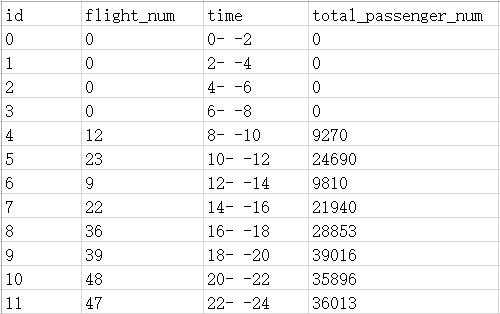
\includegraphics[width=0.7\textwidth]{figures/Data_31.png}
\caption{the data that we collected}
\label{fig:label}
\end{figure}
(The third column is the time period, the second column is the number of flights in the time period, and the fourth column is the total number of passengers in the time period)\\
For the number of people on each flight, P will choose a taxi. We check the airport traffic every 2 hours, and then based on the big data of Pudong Airport - during the day, about 15% of passengers will choose a taxi, 1.5 per car. people. In the evening, about 45% of passengers will choose a taxi, 1.5 people per car. You get the number of taxis you need every two hours, and assuming you have the same number of taxis on each flight, you can get as many taxis as you need for each flight.
Assuming that the number of taxi passengers selected on each flight is the same, you can get the number of taxis P that will be required for each flight, and the direct time interval $\Delta t$.

\begin{figure}[H]
\centering
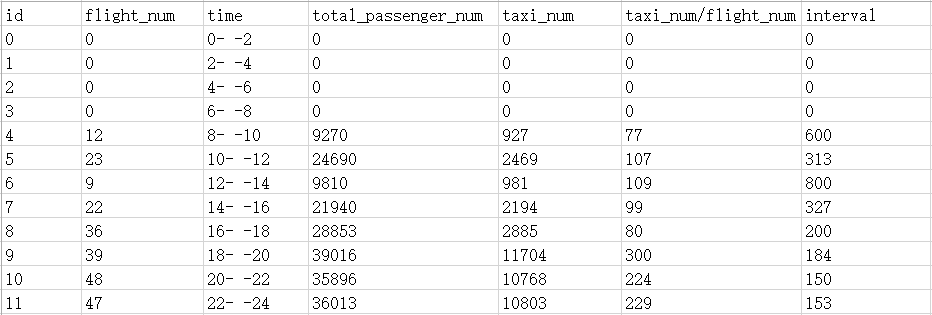
\includegraphics[width=0.7\textwidth]{figures/data3_2.png}
\caption{Flight schedule}
\label{fig:label}
\end{figure}

\item \textbf{Model calculation}\\
The initial length of the team is 0, and the airport traffic is small in the morning.
considering:
\begin{equation}\begin{split} T_{s} = \frac{{(d+k*\Delta d)}*{(n-1)}*{x}}{2}+\frac{{(d+k*\Delta d)}*{(m-1)}*{(p-x)}}{2}+t_t*(P-x)\\+\frac{{(d+k*\Delta d)}*{(n-1)}*x}{v*k}+\frac{{(d+k*\Delta d)}*{(n-1)}*(p-x)}{v*k}+\frac{c}{2}*\frac{x}{n}*\frac{x}{n*k}\\+\frac{c}{2}*\frac{P-x}{m}*+\frac{P-x}{m*k}\end{split}\end{equation}

Where d is the minimum distance of the boarding point, considering that the boarding point is relatively crowded, the taxi speed limit is 20km/h, the safety distance is 10m, take d=10, $\Delta$ d=4. There are k vehicles in the same train at the time of each batch of vehicles. Considering safety and order, they should be as small as possible. $T_t$ is the time of crossing the bridge, which is roughly set to 30s. The average speed of the taxi is considered to be 5m/s and the baggage time is 20s.
In order to find the loading point n, m and the passenger arrangement x and the taxi arrangement k which minimize the waiting time of $T_s$, the genetic algorithm is used to solve the problem. When the termination condition is reached for a certain flight, the passengers of the previous flight are still found. queue.
Substituting into the model calculation, the results are as follows. (The first column: the first flight on that day, the second column: the average number of taxis required for passengers on each flight, the third column: flight interval (seconds), the fourth column: the number of points on the L side ( n), the fifth column: the number of boarding points on the R side (m), the sixth column: the number of passengers who need to cross the bridge account for all passengers (x/p), the seventh column: the same boarding point in a group of taxis Number of cars (k), eighth column: number of queues at the pick-up point when the flight arrives (B), ninth column: model maximum number of passengers per second ($E_m$)

\begin{figure}[H]
\centering
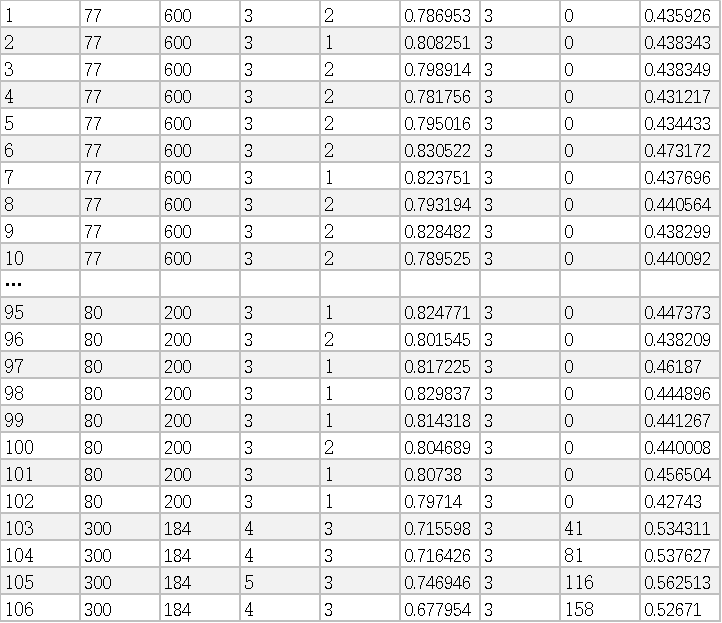
\includegraphics[width=0.7\textwidth]{figures/data3_3.png}
\caption{Calculation result table 1}
\label{fig:label}
\end{figure}

It was found that until 103 flights arrived at 6 pm, when the current flight arrived, the person on the pick-up point was waiting in line. That is, before 6 pm, all the time when the current flight arrived, it was found that there was no queue at the pick-up point. In order to minimize the total waiting time $T_s$ of all passengers, the boarding point should be arranged with 3 on the L side, 2 on the R side, and the distance between the boarding points is 18m; the vehicle arrangement is k=3, that is, each batch is rented. There are 3 consecutive vehicles to the same boarding point; passengers arrange about 1/5 passengers to pass the bridge, go to the R side to wait for the car, and let the top two of the team get on the train at the same time.
After 6 pm, the traffic volume continues to increase and reaches the peak at 22-24, using the model at this time.
\begin{equation} T_{s} = \frac{{(d+k*\Delta d)}*{(n-1)}*{(B*2*n'+p)}}{v*k}+c*\frac{2*B*n'+p}*{4*n}*{(2*B*n'+p)}\end{equation}
\begin{equation} B =B'+\frac{p}{2*n}-\frac{\Delta t*E_m}{2*n} \end{equation}
\begin{equation} v =v_1 * In[\frac{k_j}{k}]\end{equation}
The minimum distance between the vehicles on the d, considering that the boarding point is relatively crowded, the taxi speed limit is 20km / h, the safety distance is 10m, take d = 10, $\Delta$ d = 4. There are k vehicles in the same train at the time of each batch of vehicles. Considering safety and order, they should be as small as possible. The taxi speed $v_1$ considers the speed limit to be 5m/s, $k_j$ is 1/3, k=k/(10+4*k), because the passenger flow is huge at this time, so the waiter is added to serve the passengers, carry the luggage and sit on the seat. The time c is shortened to 5s.
In order to find the boarding point arrangement n and the taxi arrangement k which minimize $T_s$, that is, the waiting time, a genetic algorithm is used for solving.
Substitute the model calculation and get. (The first column: the first flight on that day, the second column: the average number of taxis required for passengers on each flight, the third column: flight interval (seconds), the fourth column: the number of passengers on one side (n ), the fifth column: the number of cars in the same boarding point in a batch of taxis (k), the sixth column: the number of people queued at the arrival point when the flight arrives (B), the seventh column: the maximum number of passengers per second in the model ( $E_m$))
\begin{figure}[H]
\centering
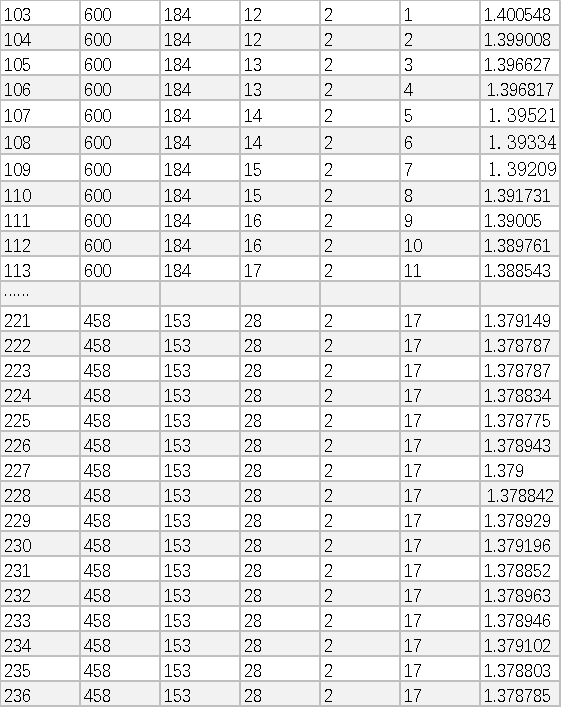
\includegraphics[width=0.7\textwidth]{figures/data3_4.png}
\caption{Calculation result table 2}
\label{fig:label}
\end{figure}
It can be seen that after 6 pm, 28 parking spots need to be arranged on the side of the road. The distance between each parking point is 122 meters. If this arrangement is arranged, the waiting team will not increase any more when it is increased to a certain length. The length is 17, because the total number is 17*33*2, and the maximum number of passengers per second is 1.358. Therefore, the last passenger can take about 15 minutes to wait until the car, and the model service capability is acceptable.
By sorting the number of points printed on the above into a picture, you can see the number of boarding points that should be arranged for each time period.
\begin{figure}[H]
\centering
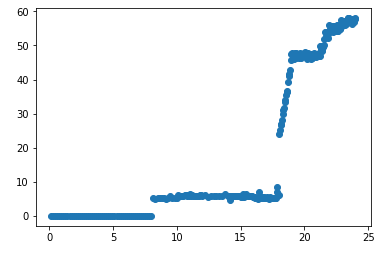
\includegraphics[width=0.7\textwidth]{figures/data3_5.png}
\caption{Boarding time period chart}
\label{fig:label}
\end{figure}
0 to 8 o'clock, the total number of boarding points is 0;
From 8:00 to 18:00, the total number of boarding points is 5, 3 on one side and 2 on the other side;
From 18 o'clock to 22:00, the total number of boarding points is 46, 23 on one side and 23 on the other side;
From 22 o'clock to 24:00, the total number of boarding points is 56, 28 on one side and 28 on the other.

\item \textbf{Model rationality analysis}\\
We found information about Pudong International Airport:\\
1. Passengers can get on the bus within an average of 20 minutes during peak hours, which is basically consistent with the model;\\
2. Pudong Airport arranged a “baggage ambassador” in uniform to help when the passenger flow was large, which was consistent with the model assumptions;\\
3. Pudong Airport will issue a card to the taxi driver to specify the driver's pick-up point to be driven, which is consistent with our model assumptions;\\
4. Pudong Airport arranged a corresponding pick-up point for each taxi, which is consistent with the model assumptions. Pudong International Airport has a maximum of 12 pick-up points, and we have calculated 56. The difference is so great. The reasons we analyzed are: the road at the pick-up point of Pudong International Airport can accommodate more than two vehicles, and the pick-up point Can be scattered in all directions of the airport; and the problem requires that the boarding point road can only accommodate two cars, and all the loading points are concentrated on one road, so our model has less space in the scheduling, in order to meet the same The magnitude of the passenger flow leads to deviations in the results.

\end{enumerate}




\section{Problem 4: Design for Priority Model}
\subsection{Construction of Priority Model}
Generally speaking, the average income of long-distance taxis is higher than that of short-distance taxis. Therefore, the following priority schemes are formulated for short-distance taxis:

A short Lane will be added in the queuing area for taxis with short-distance passengers delivering last time. The other is the general queuing lane. The vehicles in the short Lane have priority to enter the loading area for reaching passengers, and the vehicles in the general lane can only enter the loading area for boarding passengers after all the vehicles in the short Lane have been arranged. Every time the taxi finishes loading passengers from the airport, there will be mileage record. When the airport staff determines that the mileage record is a short distance, the taxi can enter the short distance lane for priority.

The following analysis shows the change of taxi revenue after the implementation of the plan:

Assume the short-distance taxis returns to the airport every time after delivering short-distance passengers. They start to line up at time $D$, board at time $E$, finish delivering at time $F$, return to the airport at time $G$. The short-distance taxis continuously delivering the short-distance passengers $i$ times in a cycle until get and deliver long-distance passenger, then the total revenue of the short-distance taxis is:
\begin{equation}
	W_{st} = I_{s} \cdot i + I_{l}, i = 1,2,3,..,N_{c}
\label{W_st}
\end{equation}
where $I_{s}$ and $I_{l}$ are the short-distance and long-distance taxi fares respectively, which are determined by the taxi charging standard and the mileage $L_{s}$ and $L_{l}$, and the net income is:
\begin{equation}
	W_{s} = W_{st} - 2 \cdot o \cdot i + O_{l}
\label{W_s}
\end{equation}
$O_{s}$ and $O_{l}$ are respectively the fuel charge for short-distance and long-distance mileage:
\begin{equation}
	O_{s} = o \cdot k + L_{s}
\label{O_s}
\end{equation}
\begin{equation}
	O_{l} = o \cdot k + L_{l}
\label{O_l}
\end{equation}
The probability that the taxi will carry the short distance passengers for $i-1$ times after the first time is:
\begin{equation}
	P(x = i)=(1-P_{l})^{i-1}\cdot P_{l}
\label{P_i}
\end{equation}
Obviously, the random variable $i$ obeys the geometric distribution. Its expectation is:
\begin{equation}
	E(X)=\frac{1}{P_{l}}
\label{E_X}
\end{equation}
The total cycle time is the time of $i$ times queues, plus the time of $i$ round trips, plus the time of the last long-distance delivery:
\begin{equation}
	t_{s2} = t_{DE} \cdot i + 2 \cdot i \cdot t_{EF} + t_{l}
\label{t_s2}
\end{equation}
$t_{EF}$ and $t_{L}$ are also related to mileage $L_{s}$ and $L_{L}$, respectively:
\begin{equation}
	t_{EF} = \frac{L_{s}}{\alpha \cdot \beta \cdot V_{1}}
\label{t_EF}
\end{equation}
\begin{equation}
	t_{l} = \frac{L_{l}}{\alpha \cdot \beta \cdot V_{1}}
\label{t_l}
\end{equation}
$t_{DE}$ is obtained by clustering analysis of flight density and taxi density in this time period. So the average hourly revenue of short distance vehicles in the cycle becomes:
\begin{equation}
	\bar{W_{s}} = \frac{I_{s}\cdot E(X)+I_{l}-2\cdot O_{s}\cdot E(X)-O_{l}}{t_{DE} \cdot E(X)+2 \cdot E(X)\cdot t_{EF}+t_{l}}
\label{W_s_bar}
\end{equation}
It is set that the long-distance taxis will not return to the airport after delivering passengers. For the long-distance bus, one cycle is queuing, carrying and finishing delivering. Assume the long-distance taxis start to queue at time $D$, carry passengers at time $E$ (the average queuing time of all the taxis is the same), and carry passengers at time $H$, then the average hourly income $\bar{W_{l}}$ of the long-distance taxi meets the requirements:
\begin{equation}
	\bar{W_{l}} = \frac{I_{l}-O_{l}}{t_{DE} +t_{EH}}
\label{W_l_bar}
\end{equation}
where
\begin{equation}
	O_{l} = o \cdot k + L_{l}
\label{O_l}
\end{equation}
\begin{equation}
	t_{EH} = t_{l}
\label{t_EH}
\end{equation}
Set the total number of taxis is $N_{C}$, and the proportion of long-distance vehicles is $P_{l}$. then, the average hourly income $W_{b}$ for every taxi  before the implementation of the plan is:
\begin{equation}
	W_{b} = \bar{W_{l}}\cdot P_{l} + \bar{W_{s}} \cdot (1 - P_{l})
\label{W_b}
\end{equation}
The variance of the average revenue is:
\begin{equation}
	S_{b} = N_{c}\cdot P_{l}\cdot (\bar{W_{l}} - W_{b})^{2} + N_{c}\cdot(1- P_{l}) \cdot (\bar{W_{s}} - W_{b})^{2}
\label{S_b}
\end{equation}
After the implementation of the plan, the cycle of the short distance vehicle is still $i$ consecutive short distance cycle plus the last long distance cycle, and its net income is the same as before the implementation of the plan:
\begin{equation}
	W_{s2} = W_{s}
\label{W_s2}
\end{equation}
After the first queue, the time of each queue is decreased, changes to:
\begin{equation}
	t_{DE2} = (1-P_{l})\cdot t_{DE}
\label{t_DE2}
\end{equation}
The total cycle time is the time of the first queue plus the time of the next $i-1$ queues plus the time of $i$ round trips plus the time of the last long-distance delivery:
\begin{equation}
	t_{s2} = t_{DE}+t_{DE2}\cdot (i-1) + 2 \cdot i \cdot t_{EF} + t_{EH}
\label{t_s2}
\end{equation}
So the average hourly revenue of short distance vehicles in the cycle becomes:
\begin{equation}
	\bar{W_{s2}} = \frac{I_{s}\cdot E(X)+I_{l}-2\cdot O_{s}\cdot E(X)-O_{l}}{t_{DE} +t_{DE2}\cdot (E(X)-1)+2 \cdot E(X)\cdot t_{EF}+t_{EH}}
\label{W_s_2}
\end{equation}
For a long-distance taxi, still assume the long-distance taxi does not turn back to the airport, the average revenue of one cycle of the long-distance taxi is:
\begin{equation}
	\bar{W_{l2}} = \bar{W_{l}}
\label{W_l2_bar}
\end{equation}
The average hourly revenue per taxi becomes:
\begin{equation}
	W_{a} = \bar{W_{l2}}\cdot P_{l} + \bar{W_{s2}} \cdot (1 - P_{l})
\label{W_a}
\end{equation}
The variance of revenue becomes:
\begin{equation}
	S_{a} = N_{c}\cdot P_{l}\cdot (\bar{W_{l2}} - W_{a})^{2} + N_{c}\cdot(1- P_{l}) \cdot (\bar{W_{s2}} - W_{a})^{2}
\label{S_b}
\end{equation}
If $S_{b}$ > $S_{a}$, it shows that our priority scheme does make the revenue of all taxis in this time period more balanced.
\subsection{Verification of Priority Model}
Similarly, Pudong Airport is selected as the actual example. The scenario is the same as the previous example with the same parameter setting of table\ref{parameter_setting}. 

For the time being, the value of $P_{l}$ cannot be obtained. Therefore, we have set multiple candidate values for $P_{l}: 0.6, 0.7, 0.8$, (set $P_{l} > 0.5$, because most airport passengers are long-distance passengers) and we observed multiple experimental results. And from these results, we can draw some conclusions:
\begin{figure}[h]
\centering
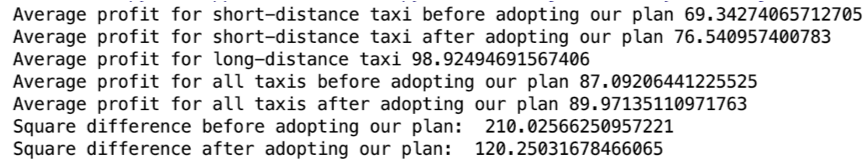
\includegraphics[width = 1.0\textwidth]{P_l6.png}
\caption{Results when $P_{l} = 0.6$}
\label{P_l6}
\end{figure}

\begin{figure}[h]
\centering
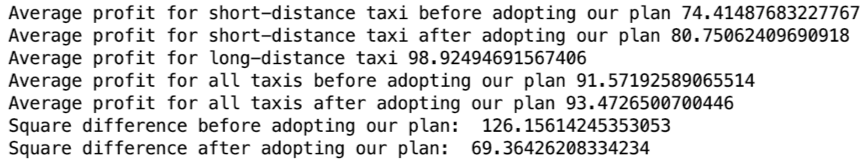
\includegraphics[width = 1.0\textwidth]{P_l7.png}
\caption{Results when $P_{l} = 0.7$}
\label{P_l7}
\end{figure}

\begin{figure}[h]
\centering
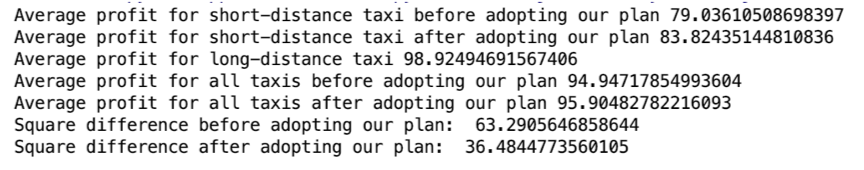
\includegraphics[width = 1.0\textwidth]{P_l8.png}
\caption{Results when $P_{l} = 0.8$}
\label{P_l8}
\end{figure}

\begin{enumerate}

\item 
This scheme can significantly reduce the variance of average revenue and make the revenue of all taxis as balanced as possible.
\item 
It is true that airport long-distance passenger transport is more profitable than short-distance passenger transport, so it is a scientific and reasonable measure to set up a priority scheme for short-distance vehicles.
\item
This scheme improves the average revenue of short distance vehicles and all taxis to a certain extent.
\item
With the increase of $P_{l}$, almost all taxis take long-distance passengers, so the variance of the overall income decreases.
\end{enumerate}
%
%
%
%\subsection{Weaknesses}
%\begin{enumerate}
%\item \textbf{Our model is just a rough model} \\
%For simplicity, we have neglected many potential parameters, variables or processes, and have made numerous assumptions. Eg. we did not consider the relationship between separate individuals and we did not dig deeper into the properties of social network which is a quite essential part determining the spread of disease. Some important general or specific factors are also neglected by us, a interesting example of which is a folk custom prevalent in the studied region that relatives kiss the death, which plays a significant role in the spread of disease and is categorized into \emph{Super Spread Event}(SSE) academically. 
%
%\item \textbf{Our model is only a continuous model} \\
%Numbers of people, number of shares of drug/vaccine, etc. are important quantities in all the process of modeling and computation. For simplicity, we regard the numbers as directly real numbers instead of integers. It is justifiable when the numbers are large, since the decimal part of the number is negligible; when the system scales down, however, the statistics dose not work and the outcome deviates a lot from reality.
%\end{enumerate}
\section{Model Appraisal}

\subsection{The strengths of the model}
In this paper, we have constructed our models based on the biological features of EVD, social features of human society and several reasonable assumptions. Our models consist of two parts: one is considering the the spread of disease within a single city and serves as the base of the other; the other takes the people flow among the cities into account, the application of which gives an optimized plan regarding how should we allocate the resources of medication such as vaccine.

\subsection{The weaknesses of the model}

Both of the models are applied to specific cases separately, and the results of computation which are carefully studied justified our model. Through our analysis of the model, we explored and explained the complex relationship among numerous variables and parameters.

\subsection{The improvement of the model}
The effectiveness of medical treatment ( including segregation, vaccination and pharmacotherapy ) is verified by our model and the strategy to allocate vaccine and drug is revealed by our investigation.

\subsection{The Extension of the model}
\section{Conclusion}

\begin{enumerate}
\item In this paper, We have established a total of three mathematical models.
\item For question 1, 2. We consider the driver's profit for the purpose, so use the airport and taxi data, through the gathering

    

Class analysis, approximation, probability statistics and other methods can quantify each influencing factor and obtain a decision model.
\item For question 3, we have to consider that the setting of the boarding point should make passengers ride the most efficient. Therefore, we will get the number and interval of boarding points and how many taxis.
And how many passengers correspond to a boarding point to establish a dynamic queuing service model for time and passenger traffic
Type, the solution method uses genetic algorithm. 
The reason is different from the actual plan.
\item For question 4, we provide a priority plan: add a short-distance lane in the queuing area for the upper
The passengers in the short-distance lanes are queued for the passengers in the short-distance lanes. For the program
Validity, we conducted modeling validation.

\end{enumerate}
\begin{thebibliography}{99}
%\addcontentsline{toc}{section}{References}

\bibitem{huang1998extensions}
Z.~Huang, ``Extensions to the k-means algorithm for clustering large data sets
  with categorical values,'' \emph{Data mining and knowledge discovery},
  vol.~2, no.~3, pp. 283--304, 1998.
\end{thebibliography}

%====================附录导入程序代码==========================================
\begin{appendices}
    %\renewcommand{\thesection}{\Alph{chapter}.}

\section{Source Codes}
Here are programmes we used in our model as follow.\\
\textbf{\textcolor[rgb]{0.98,0.00,0.00}{K-means source code:}}
\lstinputlisting[language=Python]{./code/k_means.py}
\textbf{\textcolor[rgb]{0.98,0.00,0.00}{Model2 source code:}}
\lstinputlisting[language=Python]{./code/Model2.py}
\textbf{\textcolor[rgb]{0.98,0.00,0.00}{Model4 source code:}}
\lstinputlisting[language=Python]{./code/Model4.py}

\end{appendices}

\end{document}